% 原文 printed pp.115--151 / PDF pp.130--166
\sectionlink{デコヒーレンスは至る所にある：環境散乱による局在化}
% 原文 p.115
\hypertarget{srcpage:115}{}\label{srcpage:115}
環境粒子の散乱によって誘起される局在化は、いくつかの理由から、まさにデコヒーレンスの研究計画と量子から古典への移行の核心に位置するといってよい。

環境散乱は、熱放射の放出（6.2.5節参照）と並んで、巨視的領域における支配的で遍在的なデコヒーレンス過程である。空気分子、光（可視光子）、環境放射能、宇宙線ミュー粒子、太陽ニュートリノ、さらには宇宙の至る所に存在する3\,Kの宇宙背景放射さえも、対象となる量子系の位置を絶えず監視している。その結果、系と環境の間に量子もつれが生じ、空間的に離れた波動関数成分間の局所的な位相関係が非局在化され、位置空間におけるデコヒーレンス（すなわち局在化）が起こる。精巧な実験装置を用いれば、こうした環境粒子の一部（空気分子や光など）から系を遮蔽できるかもしれないが、それ以外の影響を排除することは、不可能とまではいわなくとも、途方もなく難しい。

事実上どのような粒子による環境散乱も問題となる理由を理解するうえで、ここでもデコヒーレンスの量子的性質が重要である。第1章ですでに指摘し、2.11節でより一般的に論じたように、散乱の古典的描像では、散乱される粒子の質量が散乱体の質量に比べて十分大きい場合に限って、散乱体がその粒子の影響を受ける。簡単にいえば、ビリヤード球のNewton力学的運動を決定する際に、空気分子や光子などの影響を気にする必要はない。これに対して量子的描像では、散乱系と散乱される粒子の間のいかなる相互作用も、質量比にかかわらず、もつれを生じさせ、したがってデコヒーレンスをもたらしうる。通常、物体が巨視的になるほど散乱断面積が大きくなり、環境散乱によって、より強く、より速くデコヒーレンスが起こる。この振る舞いは、2.12節で論じたように、デコヒーレンスが、系が環境を摂動する状況に対応していることから理解できる（この過程は、今度は系の縮約された運動に影響を及ぼす）。したがって、この摂動の程度、ひいては系に導入されるデコヒーレンスの大きさが、系の大きさとともに増すことは直観的に明らかである。

% 原文 p.116
\hypertarget{srcpage:116}{}\label{srcpage:116}
環境散乱と、その結果生じる空間的局在化の過程は、歴史的な理由からも重要な役割を果たしている。位置空間の狭い波束を粒子やその軌道と直接同一視しようとする試みは、量子力学の初期にさかのぼる。フランスの物理学者Louis de Broglieは、相対性理論と光電効果から着想を得て、1920年代初頭に、質量$m$、速度$v$のあらゆる粒子には、波長$\lambda=h/mv$の量子的な「物質波」が付随すると提案した\cite{ref034,ref153,ref154,ref155}。Schrödingerは、de Broglieの1924年の博士論文\cite{ref156}から強い影響を受けていた。これは、1925年11月16日付のEinstein宛ての手紙にも表れている。
\begin{quote}
このところ私は、Louis de Broglieの独創的な理論に熱中しています。これは途方もなく刺激的ですが、なお非常に深刻な困難をいくつか抱えています。
\end{quote}
そのわずか数週間後、Schrödingerはde Broglieの物質波を波動関数$\psi$と同一視し、その波動関数の時間発展を定める有名な波動方程式を定式化した。こうして波動力学が誕生した。

しかしSchrödingerは、理論を構築するやいなや、空間的に広がった波によって粒子をどう記述するかという問題に気づいた。自由粒子については、ユニタリーな時間発展によって、空間的に局在したいかなる波束もコヒーレントに広がる傾向があることはよく知られている（図3.1）。例えば、時刻$t=0$の自由粒子が
\begin{equation}
\psi(x,t=0)=\left(\frac{1}{\sqrt{\pi}\sigma}\right)^{1/2}\exp\left[-\frac{x^2}{2\sigma^2}\right]
\tag{3.1}
\end{equation}
という波束で記述されるなら、後の時刻$t>0$での位置の確率密度$|\psi(x,t)|^2$は
\begin{equation}
\begin{aligned}
|\psi(x,t)|^2&=\frac{1}{\sqrt{\pi}\sigma[1+\hbar^2t^2/(m^2\sigma^4)]^{1/2}}
\exp\left[-\frac{x^2}{\sigma^2[1+\hbar^2t^2/(m^2\sigma^4)]}\right]\\
&\equiv\frac{1}{\sqrt{\pi}\sigma(t)}\exp\left[-\frac{x^2}{\sigma^2(t)}\right]
\end{aligned}\tag{3.2}
\end{equation}
となる。
\begin{figure}[htbp]\centering
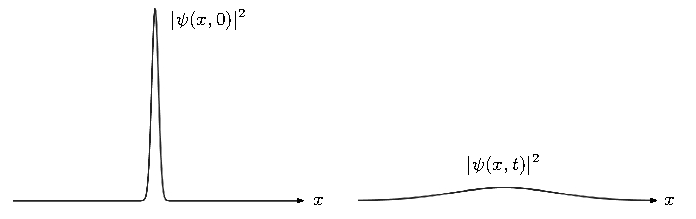
\includegraphics[width=.9\linewidth]{figures/ch03_fig01.pdf}
\caption{ユニタリーな時間発展に伴う、自由粒子のGaussian波束の確率密度$|\psi(x,t)|^2$のコヒーレントな拡散。}\label{fig:3.1}
\end{figure}

% 原文 p.117
\hypertarget{srcpage:117}{}\label{srcpage:117}
これは、波束の幅$\sigma$が
\begin{equation}
\sigma(t)=\sigma\left[1+\hbar^2t^2/(m^2\sigma^4)\right]^{1/2}
\tag{3.3}
\end{equation}
のように増大することを意味する。微視的粒子では、この拡散は非常に短い時間で起こる。例えば、Gaussian波束が電子の質量（$m\approx10^{-30}\,\mathrm{kg}$）をもつ粒子を記述し、その初期幅が$\sigma=1\,\text{\AA}$なら、ユニタリーな時間発展によって、わずか1秒のうちに波束の幅は$10^{16}\sigma=10^6\,\mathrm{m}$程度（実に1,000\,km！）にまで広がる。自由粒子の波動関数がコヒーレントに広がるこの効果は、狭い波束を粒子と結びつけようとする立場に重大な困難をもたらした。量子力学的な波束が直ちに巨視的距離にわたってコヒーレントに分散してしまうのであれば、明らかに空間的に明確な領域内にとどまる物体を、どうしてそのような波束と直接同一視できるだろうか。

孤立した自由粒子の場合には、波束と粒子の一対一対応を確立する試みが失敗したため、Schrödingerは粒子がポテンシャルを受ける状況に注意を向けた。特に、「微視的力学から巨視的力学への連続的移行」と題する有名な1926年の論文\footnote{ドイツ語の原題は ``Der stetige Übergang von der Mikro- zur Makromechanik.'' である。}\cite{ref157}では、量子調和振動子を例に取り、位置空間でのSchrödinger方程式の解（個々には空間的に広がった波を表す）を特定の仕方で線形結合すると、得られる波束は$t=0$で狭いだけでなく、その後のすべての時刻$t>0$でも狭いままにとどまり、そのピークが古典的な質点と同じように往復振動することを示した。

もちろんSchrödingerが発見したのは、量子調和振動子のコヒーレント状態、すなわち位相空間で古典軌道に従う最小不確定性波束であった。この成功に勇気づけられ、Schrödingerは次のように予測した\cite[p.~666]{ref157}。
\begin{quote}
ほぼ同じ方法で、大きな量子数をもつ楕円形のKepler軌道をたどり、水素原子中の電子の波動力学的な姿を表す波束も構成できるだろう。ただし、ここで扱った特に簡単な例に比べて、より多くの数学的困難に遭遇するかもしれない。\footnote{ドイツ語の原文は次のとおりである。``Es läßt sich mit Bestimmtheit voraussehen, daß man auf ganz ähnliche Weise auch die Wellengruppen konstruieren kann, welche auf hochquantigen Keplerellipsen umlaufen und das undulationsmechanische Bild des Wasserstoffelektrons sind; nur sind da die rechentechnischen Schwierigkeiten größer als in dem hier behandelten, ganz besonders einfachen Schulbeispiel.''}
\end{quote}

% 原文 p.118
\hypertarget{srcpage:118}{}\label{srcpage:118}
しかし、この評価（結局のところ、楽観的すぎた評価\footnote{Kepler軌道の場合には、理想化された量子調和振動子の例のような厳密なコヒーレント状態は得られない。別の興味深い例は、カオス的な回転運動を示すことが観測されているSaturnの衛星Hyperionである。カオス的運動は、古典軌道が初期の位相空間パラメータに指数関数的に敏感であることを意味するが、Heisenbergの不確定性原理のため、それらのパラメータを任意の精度で指定することはできない。したがって、Hyperionを記述する初めは狭い位相空間波束も、非常に速く広い空間領域へ広がる。実際、Zurek\cite{ref158}は、約20年のうちに、量子状態がこの衛星の主軸の巨視的に区別できる向きの、きわめて非局所的なコヒーレントな重ね合わせになると見積もった。したがって、惑星規模でさえコヒーレントな拡散の問題が生じうる。}であった）は、先に見いだされた核心的な問題、すなわち自由粒子を波束でどう記述するかという問題には触れていない。Schrödingerの論文の発表から数十年後、量子系が開いていることの重要性と、そこから生じるデコヒーレンス効果が理解されたこと\cite{ref004,ref005,ref006,ref008,ref009,ref012}により、自由粒子についてのSchrödinger方程式の予測と、すべての巨視的物体が局在して見えるという事実をどう両立させるかという困難の解決に、大きく近づいた。JoosとZehの先駆的論文\cite{ref007}は、詳細な模型と数値的結果を通じて、光子、空気分子、その他の環境粒子による遍在的な散乱が、極端に短い時間でコヒーレントな拡散を実効的に抑制する仕組みを示した。このデコヒーレンス過程によって得られる系の縮約密度行列は、位置空間の波束の（非真正な）アンサンブルを表し、その波束の幅は熱的de Broglie波長(2.114)へ向かって急速に減少する。

以下では、JoosとZehの原模型\cite{ref007}にさかのぼる、散乱によるデコヒーレンスの模型を調べる。現在では、文献\cite{ref007}に示された縮約密度行列の運動方程式の導出には微妙な誤りがあり、その結果、デコヒーレンス率が正しい値より$2\pi$倍大きくなることがわかっている\cite{ref159,ref160,ref161}。もちろん、論文が発表された1985年には、このような時間尺度の測定はいかなる実験でも手の届かないものに思われたため、JoosとZehの関心は、デコヒーレンスの時間尺度の簡単な見積もりにあった。しかし、この数年の実験技術の急速な進歩により、巨視的あるいは中間的な大きさの物体についてさえ、デコヒーレンスの時間尺度をきわめて精密に測定できるようになった（例えば、6.2節で述べるC$_{70}$分子の干渉実験を参照）。これらの測定は、前述の$2\pi$という因子程度の違いにも敏感であるため、定量的に正しい結果を与える環境散乱理論を用いることが重要になった。

さらに、JoosとZehの元の研究は、物体と散乱される環境粒子の波長の相対的な大きさについての仮定に基づいていた。この仮定を緩めた、より一般的な方法が、その後GallisとFleming\cite{ref162}によって与えられたが、導出における前述の誤りには対処しておらず、依然として余分な誤った因子$2\pi$が残った。

% 原文 p.119
\hypertarget{srcpage:119}{}\label{srcpage:119}
この誤りを修正し、デコヒーレンス率について正しい結果に到達した最初の導出は、Diósi\cite{ref159}によって与えられた。その数年後、HornbergerとSipe\cite{ref160}は環境散乱の問題を再検討し、Diósiのものとは大きく異なる洗練された方法を用いて正しい結果を得た。彼らの再評価は非常に注意深く徹底している一方で、かなり複雑でもある。最近、Adler\cite{ref161}は、ちょっとした工夫によって、はるかに簡単に正しい結果を得られることを示した。そのほか、例えばHalliwell\cite{ref163}やHornberger\cite{ref164,ref165}による導出もある。以下では、計算をできるだけ簡単に保ちながら正しい結果を得ることを目指して、主にHornbergerとSipe\cite{ref160}およびAdler\cite{ref161}の導出に従う。

本章の構成は次のとおりである。3.1節では散乱模型を導入する。3.2節では、空間的コヒーレンスの減衰を記述するデコヒーレンス因子の具体的な形を計算する。3.3節では二つの重要な極限、すなわち、系の空間的重ね合わせ状態を構成する二つの重心位置のコヒーレントな隔たりと比べて、環境の波長が短い場合（3.3.1節）と長い場合（3.3.2節）を扱う。3.4節では、この理論を光子の散乱（3.4.1節）と空気分子の散乱（3.4.2節）に適用する。最後に3.5節では、系の縮約密度行列の時間発展を調べることで、このような散乱によるデコヒーレンスから生じる具体的な運動を論じる。

\subsectionlink{散乱模型}
ある物体（系S）が、多数の環境粒子（環境E）を散乱する状況を考える（図3.2）。SとEは初め完全に無相関である、すなわち複合系SEの（純粋状態の）密度行列$\hat\rho$は$t=0$で因数分解されるという、通常の仮定を置く。
\begin{equation}
\hat\rho(0)=\hat\rho_{\mathrm S}(0)\otimes\hat\rho_{\mathrm E}(0).
\tag{3.4}
\end{equation}
まず一回の散乱事象を考え、それが系の密度行列$\hat\rho_{\mathrm S}$に及ぼす影響を調べよう（図3.3）。以下では、ごく基本的な量子力学の散乱理論を用いる。この主題の解説は、量子力学の教科書の多くにある（例えば文献\cite{ref058}の第7章）。しかし、他の文献を参照しなくても、読者はこの導出を追えるはずである。

重心位置$\bm x$をもつ系の初期状態を、固有値$\bm x$の位置固有状態$|\bm x\rangle$で表し、入射する環境粒子の初期状態を$|\chi_{\mathrm i}\rangle$と書こう。すると、散乱事象の効果は、散乱演算子$\hat S$（いわゆる「S行列」）の初期状態への作用によって、形式的に
\begin{equation}
|\bm x\rangle|\chi_{\mathrm i}\rangle\longrightarrow\hat S|\bm x\rangle|\chi_{\mathrm i}\rangle
\tag{3.5}
\end{equation}
と表せる。ここでは初期状態に対する分離可能性の仮定(3.4)を用いた。

\begin{figure}[htbp]\centering
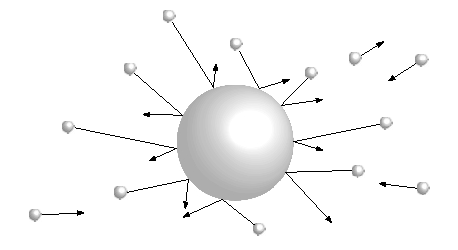
\includegraphics[width=.58\linewidth]{figures/ch03_fig02.pdf}
\caption{環境散乱。光子や空気分子などの粒子の集まりが、対象となる物体によって散乱される。}\label{fig:3.2}
\end{figure}
\begin{figure}[htbp]\centering
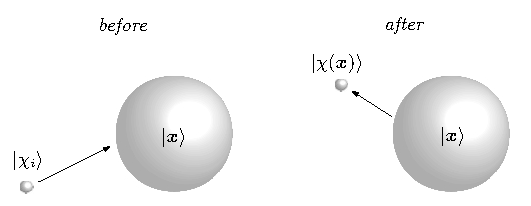
\includegraphics[width=.8\linewidth]{figures/ch03_fig03.pdf}
\caption{一回の散乱事象。初期状態$|\chi_{\mathrm i}\rangle$で記述される入射環境粒子が、静止した対象物によって弾性散乱される。対象物の重心状態は位置固有状態$|\bm x\rangle$で表される。散乱ポテンシャルの到達範囲は十分短く、物体と入射粒子の状態は初め無相関である。物体は散乱される環境粒子よりはるかに重く、散乱事象によって乱されないと仮定する。したがって、この相互作用は$|\bm x\rangle|\chi_{\mathrm i}\rangle\longrightarrow|\bm x\rangle|\chi(\bm x)\rangle$という発展をもたらす。$|\chi(\bm x)\rangle$は散乱粒子の終状態である［(3.12)も参照］。}\label{fig:3.3}
\end{figure}

% 原文 p.120
\hypertarget{srcpage:120}{}\label{srcpage:120}
自明なことを述べる危険を承知で付け加えれば、もちろん$|\chi_{\mathrm i}\rangle$は散乱物体の位置$\bm x$に依存しない。状態$|\bm x\rangle$は、原点に散乱中心がある状態$|\bm x=0\rangle$を、系の運動量演算子$\hat{\bm p}$の作用によって平行移動したものと考えられる。\footnote{この模型はデコヒーレンス時間尺度の具体的な数値の計算に用いるため、以下の導出では$\hbar$を残す。}
\begin{equation}
|\bm x\rangle=e^{-\mathrm i\hat{\bm p}\cdot\bm x/\hbar}|\bm x=0\rangle.
\tag{3.6}
\end{equation}
したがって(3.5)を次のように書き換えられる。
\begin{equation}
e^{-\mathrm i\hat{\bm p}\cdot\bm x/\hbar}|0\rangle|\chi_{\mathrm i}\rangle
\longrightarrow\hat S e^{-\mathrm i\hat{\bm p}\cdot\bm x/\hbar}|0\rangle|\chi_{\mathrm i}\rangle
=\hat S e^{-\mathrm i(\hat{\bm p}+\hat{\bm q})\cdot\bm x/\hbar}|0\rangle e^{\mathrm i\hat{\bm q}\cdot\bm x/\hbar}|\chi_{\mathrm i}\rangle.
\tag{3.7}
\end{equation}
% 原文 p.121
\hypertarget{srcpage:121}{}\label{srcpage:121}
ここで$\hat{\bm q}$は散乱される粒子の運動量演算子であり、したがって$\hat{\bm P}\equiv\hat{\bm p}+\hat{\bm q}$は複合系SEの運動量演算子である。

散乱相互作用が、複合系SEの空間的平行移動（すなわち演算子$\hat{\bm P}$が生成する平行移動）に対して不変である、
\begin{equation}
[\hat S,\hat{\bm P}]=0
\tag{3.8}
\end{equation}
と仮定すると、(3.7)の右辺の最初の指数関数を前に出して
\begin{equation}
\hat S|\bm x\rangle|\chi_{\mathrm i}\rangle
=e^{-\mathrm i(\hat{\bm p}+\hat{\bm q})\cdot\bm x/\hbar}\hat S|0\rangle e^{\mathrm i\hat{\bm q}\cdot\bm x/\hbar}|\chi_{\mathrm i}\rangle
\tag{3.9}
\end{equation}
を得る。

さらに進むため、ここで重要な仮定を置く。物体と散乱粒子の相互作用によって物体に反跳が生じないとするのである。これは、粒子が散乱事象によって実質的に乱されず、したがって散乱過程の唯一の帰結が、系と環境の間に量子的相関（もつれ）を作ることであることを意味する。

この仮定は、散乱系が散乱粒子よりはるかに重く、系の反跳効果を無視できる状況ではよい近似となる。微視的または中間的な大きさの粒子が巨視的物体によって散乱される場合には、これが成立すると期待できる。しかし、文献に挙げられた空間的デコヒーレンスの時間尺度の中には、散乱物体と散乱される環境粒子との質量比が1に近いか、あるいは1未満である散乱過程にも、この仮定を適用して計算したものがあることに注意しよう。一例は、空気分子の散乱によってデコヒーレンスを起こす小さな分子や自由電子の場合である\cite{ref166}。明らかに、この領域では無反跳の仮定が物理的に現実的であるとは期待できず、したがって（反跳を考慮する）Diósiの模型\cite{ref159}のような、より一般的な模型に頼るべきである。

以下の扱いでは、散乱物体が環境粒子よりはるかに重いとすることで、上の無反跳散乱の仮定を採用する。すると、系と環境の複合状態に対するS行列の作用は、系の重心状態$|\bm x\rangle$に影響を与えず、重心は位置$\bm x$にとどまる。したがって(3.7)をさらに計算できる。
\begin{equation}
\begin{aligned}
\hat S|\bm x\rangle|\chi_{\mathrm i}\rangle
&=e^{-\mathrm i(\hat{\bm p}+\hat{\bm q})\cdot\bm x/\hbar}|0\rangle\hat S_0e^{\mathrm i\hat{\bm q}\cdot\bm x/\hbar}|\chi_{\mathrm i}\rangle\\
&=e^{-\mathrm i\hat{\bm p}\cdot\bm x/\hbar}|0\rangle e^{-\mathrm i\hat{\bm q}\cdot\bm x/\hbar}\hat S_0e^{\mathrm i\hat{\bm q}\cdot\bm x/\hbar}|\chi_{\mathrm i}\rangle\\
&=|\bm x\rangle e^{-\mathrm i\hat{\bm q}\cdot\bm x/\hbar}\hat S_0e^{\mathrm i\hat{\bm q}\cdot\bm x/\hbar}|\chi_{\mathrm i}\rangle.
\end{aligned}\tag{3.10}
\end{equation}
ここでは散乱演算子$\hat S$に添字「0」を加え、散乱中心が原点にある散乱過程を特に指す演算子であることを示した。

% 原文 p.122
\hypertarget{srcpage:122}{}\label{srcpage:122}
(3.10)の最後の行を用いて、平行移動された散乱演算子
\begin{equation}
\hat S_{\bm x}\equiv e^{-\mathrm i\hat{\bm q}\cdot\bm x/\hbar}\hat S_0e^{\mathrm i\hat{\bm q}\cdot\bm x/\hbar}
\tag{3.11}
\end{equation}
を定義できる。これは散乱中心が位置$\bm x$にある散乱を記述する。まとめると、散乱相互作用は
\begin{equation}
|\bm x\rangle|\chi_{\mathrm i}\rangle\longrightarrow\hat S|\bm x\rangle|\chi_{\mathrm i}\rangle
=|\bm x\rangle\hat S_{\bm x}|\chi_{\mathrm i}\rangle\equiv|\bm x\rangle|\chi(\bm x)\rangle
\tag{3.12}
\end{equation}
と与えられる。ここで$|\chi(\bm x)\rangle$は、$\bm x$で散乱された環境粒子の終状態の略記である。(3.12)から、散乱過程は、系の重心位置を記述する状態$|\bm x\rangle$と、散乱中心の位置$\bm x$についての経路情報を符号化した粒子の終状態$|\chi(\bm x)\rangle$の間に相関を確立する、測定に似た相互作用と考えられることがわかる。

(3.12)より、散乱過程は初期の複合密度行列
\begin{equation}
\hat\rho(0)=\hat\rho_{\mathrm S}(0)\otimes\hat\rho_{\mathrm E}(0)
=\int\mathrm d\bm x\int\mathrm d\bm x'\,\rho_{\mathrm S}(\bm x,\bm x',0)|\bm x\rangle\langle\bm x'|\otimes|\chi_{\mathrm i}\rangle\langle\chi_{\mathrm i}|
\tag{3.13}
\end{equation}
を密度行列
\begin{equation}
\hat\rho=\int\mathrm d\bm x\int\mathrm d\bm x'\,\rho_{\mathrm S}(\bm x,\bm x',0)|\bm x\rangle\langle\bm x'|\otimes|\chi(\bm x)\rangle\langle\chi(\bm x')|
\tag{3.14}
\end{equation}
に変換する。(2.50)を用いると、対応する系の最終縮約密度行列$\hat\rho_{\mathrm S}$は
\begin{equation}
\hat\rho_{\mathrm S}=\operatorname{Tr}_{\mathrm E}\hat\rho
=\int\mathrm d\bm x\int\mathrm d\bm x'\,\rho_{\mathrm S}(\bm x,\bm x',0)|\bm x\rangle\langle\bm x'|\langle\chi(\bm x')|\chi(\bm x)\rangle
\tag{3.15}
\end{equation}
と与えられる。したがって、位置基底で表すと、散乱による縮約密度行列の発展は
\begin{equation}
\rho_{\mathrm S}(\bm x,\bm x',0)\longrightarrow\rho_{\mathrm S}(\bm x,\bm x',0)\langle\chi(\bm x')|\chi(\bm x)\rangle
\tag{3.16}
\end{equation}
とまとめられる。散乱事象による空間的コヒーレンスの局所的抑制は、散乱粒子の相対状態の重なり$\langle\chi(\bm x')|\chi(\bm x)\rangle$によって定量化されることがわかる（2.6.3節と2.7節での一般的な議論も参照）。次に、この重なりの時間依存性を計算しよう。
\subsectionlink{デコヒーレンス因子の計算}
先に進むため、散乱演算子$\hat S_0$を、別の演算子$\hat T$（「T行列」）を用いて形式的に
\begin{equation}
\hat S_0=\hat I+\mathrm i\hat T
\tag{3.17}
\end{equation}
と書こう。
% 原文 p.123
\hypertarget{srcpage:123}{}\label{srcpage:123}
T行列は標準的な量子力学の散乱理論でよく知られている（例えば文献\cite{ref058}）。ここでこれを用いるのは、散乱粒子の運動量固有基底$\{|\bm q\rangle\}$における行列要素を、散乱振幅$f(\bm q,\bm q')$によって、都合よく
\begin{equation}
\langle\bm q|\hat T|\bm q'\rangle=\frac{\mathrm i}{2\pi\hbar q}\delta(q-q')f(\bm q,\bm q')
=\frac{\mathrm i}{2\pi\hbar m}\delta(E-E')f(\bm q,\bm q')
\tag{3.18}
\end{equation}
と定義できるからである。ここで$m$は環境粒子の質量、$q=|\bm q|$である。項$\delta(E-E')$は、反跳のない弾性散乱という仮定が要求するエネルギー保存を保証する。$|f(\bm q,\bm q')|^2$は実験で測定できる量、すなわち散乱過程の微分断面積$\mathrm d\sigma/\mathrm d\Omega$であり、
\begin{equation}
\frac{\mathrm d\sigma}{\mathrm d\Omega}\equiv\frac{\text{散乱流束}}{\text{入射流束}}
\tag{3.19}
\end{equation}
と定義されることに注意しよう。

散乱演算子$\hat S_0$はユニタリーであり、
\begin{equation}\hat S_0\hat S_0^{\dagger}=\hat I,\tag{3.20}\end{equation}
T行列の定義(3.17)から次の関係を得る。
\begin{equation}\hat T\hat T^{\dagger}+\mathrm i(\hat T-\hat T^{\dagger})=0.\tag{3.21}\end{equation}
この結果は後で役に立つ。

環境状態の表式(3.12)を用いると、重なり$\langle\chi(\bm x')|\chi(\bm x)\rangle$は
\begin{equation}
\langle\chi(\bm x')|\chi(\bm x)\rangle=\langle\chi_{\mathrm i}|\hat S_{\bm x'}^{\dagger}\hat S_{\bm x}|\chi_{\mathrm i}\rangle
\tag{3.22}
\end{equation}
と与えられる。明らかにこの表式は、平行移動された散乱演算子(3.11)の積$\hat S_{\bm x'}^{\dagger}\hat S_{\bm x}$の、入射環境粒子の（純粋）状態$|\chi_{\mathrm i}\rangle$における期待値に等しい（混合状態への一般化は容易である）。したがって、トレース則(2.17)を用いれば、(3.22)を同値な形
\begin{equation}
\langle\chi(\bm x')|\chi(\bm x)\rangle=\operatorname{Tr}_{\mathrm E}\{\hat\rho_{\mathrm E}(0)\hat S_{\bm x'}^{\dagger}\hat S_{\bm x}\}
\tag{3.23}
\end{equation}
に書き換えられる。ここで$\hat\rho_{\mathrm E}(0)=|\chi_{\mathrm i}\rangle\langle\chi_{\mathrm i}|$である。これがこれから計算する対象の表式である。まず、環境粒子が箱型規格化の体積$V$に制限されていると仮定しよう。文献\cite{ref160}に従い、体積$V$で規格化された運動量固有ケット$|\widetilde{\bm q}\rangle$を
\begin{equation}
|\widetilde{\bm q}\rangle\equiv\left[\frac{(2\pi\hbar)^3}{V}\right]^{1/2}|\bm q\rangle
\tag{3.24}
\end{equation}
と定義する。

% 原文 p.124
\hypertarget{srcpage:124}{}\label{srcpage:124}
ケット$|\widetilde{\bm q}\rangle$は、
\begin{equation}
\sum_{\bm q\in Q_V}|\widetilde{\bm q}\rangle\langle\widetilde{\bm q}|=\hat I_V
\tag{3.25}
\end{equation}
という意味で、体積$V$上の正規直交基底を構成する。ここで$Q_V$は、体積$V$において周期的境界条件を満たす波動関数の空間に対応するすべての運動量の集合であり、$\hat I_V$はこの空間の恒等演算子である。

すると、環境粒子の初期密度行列$\hat\rho_{\mathrm E}(0)$を、規格化された運動量固有状態$|\widetilde{\bm q}\rangle$のアンサンブルによって
\begin{equation}
\hat\rho_{\mathrm E}(0)=\frac{(2\pi\hbar)^3}{V}\sum_{\bm q\in Q_V}\mu(\bm q)|\widetilde{\bm q}\rangle\langle\widetilde{\bm q}|
\tag{3.26}
\end{equation}
と展開できる。$\mu(\bm q)$は運動量空間の密度である。この展開を用いる大きな利点は、演算子$\hat T$［(3.17)、(3.18)参照］が、全空間の運動量基底$\{|\bm q\rangle\}$で対角的であり、したがって適切に規格化された体積$V$の基底$\{|\widetilde{\bm q}\rangle\}$でも対角的であるということである。

この性質により、重なり$\langle\chi(\bm x')|\chi(\bm x)\rangle$［(3.23)参照］をかなり直接的に計算できる。(3.23)に環境状態の展開(3.26)を用いると、まず
\begin{equation}
\begin{aligned}
\langle\chi(\bm x')|\chi(\bm x)\rangle
&=\frac{(2\pi\hbar)^3}{V}\sum_{\bm q\in Q_V}\mu(\bm q)\langle\widetilde{\bm q}|\hat S_{\bm x'}^{\dagger}\hat S_{\bm x}|\widetilde{\bm q}\rangle\\
&=\frac{(2\pi\hbar)^3}{V}\sum_{\bm q\in Q_V}\mu(\bm q)\langle\widetilde{\bm q}|e^{-\mathrm i\hat{\bm q}\cdot\bm x'/\hbar}\hat S_0^{\dagger}
e^{-\mathrm i\hat{\bm q}\cdot(\bm x-\bm x')/\hbar}\hat S_0e^{\mathrm i\hat{\bm q}\cdot\bm x/\hbar}|\widetilde{\bm q}\rangle\\
&=\frac{(2\pi\hbar)^3}{V}\sum_{\bm q\in Q_V}\mu(\bm q)e^{\mathrm i\bm q\cdot(\bm x-\bm x')/\hbar}
\langle\widetilde{\bm q}|\hat S_0^{\dagger}e^{-\mathrm i\hat{\bm q}\cdot(\bm x-\bm x')/\hbar}\hat S_0|\widetilde{\bm q}\rangle
\end{aligned}\tag{3.27}
\end{equation}
を得る。次に、$\hat S_0=\hat I+\mathrm i\hat T$［(3.17)参照］および関係(3.21)を用いると、これは
\begin{equation}
\begin{aligned}
&\langle\chi(\bm x')|\chi(\bm x)\rangle\\
&=\frac{(2\pi\hbar)^3}{V}\sum_{\bm q\in Q_V}\mu(\bm q)e^{\mathrm i\bm q\cdot(\bm x-\bm x')/\hbar}
\langle\widetilde{\bm q}|(\hat I-\mathrm i\hat T^{\dagger})e^{-\mathrm i\hat{\bm q}\cdot(\bm x-\bm x')/\hbar}(\hat I+\mathrm i\hat T)|\widetilde{\bm q}\rangle\\
&=\frac{(2\pi\hbar)^3}{V}\sum_{\bm q\in Q_V}\mu(\bm q)
\left[1-\langle\widetilde{\bm q}|\hat T\hat T^{\dagger}|\widetilde{\bm q}\rangle
+e^{\mathrm i\bm q\cdot(\bm x-\bm x')/\hbar}\langle\widetilde{\bm q}|\hat T^{\dagger}e^{-\mathrm i\hat{\bm q}\cdot(\bm x-\bm x')/\hbar}\hat T|\widetilde{\bm q}\rangle\right]
\end{aligned}\tag{3.28}
\end{equation}
となる。演算子$\hat T$が運動量演算子と可換なので［(3.18)参照］、最後の行の角括弧内の第2項に付随する指数関数はすべて消えている。

% 原文 p.125
\hypertarget{srcpage:125}{}\label{srcpage:125}
運動量固有状態$|\widetilde{\bm q}\rangle$の完全系［(3.25)参照］を挿入し、さらに(3.18)を用いて、(3.28)の最後の行の和に含まれる第2項と第3項を計算しよう。すると
\begin{equation}
\begin{aligned}
&\langle\chi(\bm x')|\chi(\bm x)\rangle\\
&=\frac{(2\pi\hbar)^3}{V}\sum_{\bm q\in Q_V}\mu(\bm q)
\left[1-\sum_{\bm q'\in Q_V}\left(1-e^{\mathrm i(\bm q-\bm q')\cdot(\bm x-\bm x')/\hbar}\right)
\left|\langle\widetilde{\bm q}|\hat T|\widetilde{\bm q}'\rangle\right|^2\right]
\end{aligned}\tag{3.29}
\end{equation}
を得る。ここで、通常の変換関係
\begin{equation}
\frac{(2\pi\hbar)^3}{V}\sum_{\bm q\in Q_V}\longrightarrow\int\mathrm d\bm q
\tag{3.30}
\end{equation}
に従って和を積分に置き換え、運動量状態$|\widetilde{\bm q}\rangle$の連続極限へ移る。$\int\mathrm d\bm q\,\mu(\bm q)=1$と定義(3.24)を用いると、(3.29)は
\begin{equation}
\begin{aligned}
\langle\chi(\bm x')|\chi(\bm x)\rangle
=1-&\int\mathrm d\bm q\,\mu(\bm q)\frac{(2\pi\hbar)^3}{V}\int\mathrm d\bm q'\,
\left(1-e^{\mathrm i(\bm q-\bm q')\cdot(\bm x-\bm x')/\hbar}\right)
|\langle\bm q|\hat T|\bm q'\rangle|^2
\end{aligned}\tag{3.31}
\end{equation}
となる。

Adlerの方法\cite{ref161}に従い、散乱過程で経過した時間を表す時間パラメータ$T$を導入しよう。すると(3.16)と(3.31)から、縮約密度行列の発展は
\begin{equation}
\begin{aligned}
&\rho_{\mathrm S}(\bm x,\bm x',T)-\rho_{\mathrm S}(\bm x,\bm x',0)=-\rho_{\mathrm S}(\bm x,\bm x',0)\\
&\quad\times\int\mathrm d\bm q\,\mu(\bm q)\frac{(2\pi\hbar)^3}{V}\int\mathrm d\bm q'\,
\left(1-e^{\mathrm i(\bm q-\bm q')\cdot(\bm x-\bm x')/\hbar}\right)|\langle\bm q|\hat T|\bm q'\rangle|^2
\end{aligned}\tag{3.32}
\end{equation}
と書ける。(3.32)を書く際、物体の自由発展の特徴的な時間尺度は散乱事象の平均間隔よりはるかに長く、区間$T$内での物体の密度行列の変化は散乱事象のみから生じると仮定したことに注意しよう。

次に、この式に現れる行列要素の二乗$|\langle\bm q|\hat T|\bm q'\rangle|^2$を計算する。(3.18)の形
\begin{equation}
\langle\bm q|\hat T|\bm q'\rangle=\frac{\mathrm i}{2\pi\hbar m}\delta(E-E')f(\bm q,\bm q')
\tag{3.33}
\end{equation}
を用いると、計算すべきものは
\begin{equation}
|\langle\bm q|\hat T|\bm q'\rangle|^2=\frac{1}{(2\pi\hbar m)^2}\delta^2(E-E')|f(\bm q,\bm q')|^2
\tag{3.34}
\end{equation}
である。

% 原文 p.126
\hypertarget{srcpage:126}{}\label{srcpage:126}
エネルギーのデルタ関数の二乗$\delta^2(E-E')$は、時間依存摂動論における遷移確率についてのFermiの黄金律を導く際によく現れる（例えば文献\cite{ref167}の第18章を参照）。実際、行列要素$|\langle\bm q|\hat T|\bm q'\rangle|^2$は、明らかに散乱による遷移$|\bm q\rangle\longrightarrow|\bm q'\rangle$の確率にほかならない。

そこで、Adlerが提案した方法\cite{ref161}（Fermiの黄金律の導出に通常用いられる方法に似ている）に従い、エネルギーのデルタ関数のFourier積分表示
\begin{equation}
\delta(E-E')=\lim_{T\to\infty}\frac{1}{2\pi\hbar}\int_{-T/2}^{T/2}\mathrm dt\,e^{\mathrm i(E-E')t/\hbar}
\tag{3.35}
\end{equation}
を用いて、その二乗を扱える。これにより
\begin{equation}
\begin{aligned}
\delta^2(E-E')
&=\delta(E-E')\lim_{T\to\infty}\frac{1}{2\pi\hbar}\int_{-T/2}^{T/2}\mathrm dt\,e^{\mathrm i(E-E')t/\hbar}\\
&=\delta(E-E')\lim_{T\to\infty}\frac{1}{2\pi\hbar}\int_{-T/2}^{T/2}\mathrm dt\\
&=\delta(E-E')\lim_{T\to\infty}\frac{T}{2\pi\hbar}
\end{aligned}\tag{3.36}
\end{equation}
と書ける。第2行では、積分の前にある最初のデルタ関数が、$E=E'$でなければゼロになることを用いた。

Fermiの黄金律の一般的導出では、パラメータ$T$は、相互作用が「入っている」時間区間と解釈できる。(3.36)は、十分大きな$T$に対して遷移確率が$T$にほぼ比例して増加することを示す。したがって、$T$を一回の散乱事象が起こる典型的な所要時間よりはるかに長い時間区間とすれば、(3.36)を
\begin{equation}
\delta^2(E-E')=\delta(E-E')\frac{T}{2\pi\hbar}
=\delta(q-q')\frac{m}{q}\frac{T}{2\pi\hbar}
\tag{3.37}
\end{equation}
と書ける。さらに、$T$は、多数の粒子の散乱によって中心粒子に生じる特徴的なデコヒーレンス時間よりも十分短いと仮定する。一般に、顕著な空間的デコヒーレンスを生じるには物体と環境粒子との多数回の衝突が必要なので、このような$T$の領域を選ぶことは妥当である。

次に(3.37)を(3.34)で用い、得られた表式を(3.32)へ代入する。(3.37)のデルタ関数$\delta(q-q')$は、$|\bm q'|=|\bm q|$という運動量の保存を課す。$\mathrm d\bm q'\equiv q^2\mathrm d\hat{\bm n}'$と書くと（$\mathrm d\hat{\bm n}'$は運動量空間の立体角の微分）、容易に
\begin{equation}
\begin{aligned}
&\rho_{\mathrm S}(\bm x,\bm x',T)-\rho_{\mathrm S}(\bm x,\bm x',0)=-\rho_{\mathrm S}(\bm x,\bm x',0)\\
&\quad\times\frac{T}{V}\int\mathrm d\bm q\,\mu(\bm q)v(q)\int\mathrm d\hat{\bm n}'
\left(1-e^{\mathrm i(\bm q-q\hat{\bm n}')\cdot(\bm x-\bm x')/\hbar}\right)|f(\bm q,q\hat{\bm n}')|^2
\end{aligned}\tag{3.38}
\end{equation}
を得る。

% 原文 p.127
\hypertarget{srcpage:127}{}\label{srcpage:127}
ここで$v(q)$は、運動量$q$をもつ粒子の速さを表す。質量をもつ粒子の散乱では$v(q)=q/m$、光子など質量のない粒子の散乱では$v(q)=c$であり、$c$は光速である。

(3.38)は一回の散乱事象の効果を記述する。$N$回の独立な散乱事象の集まりは、(3.38)の右辺の積分に$N$を掛けるだけで表せる。このとき$N/V$が環境粒子の全数密度となる。簡単のため、入射粒子は空間的に等方分布している、すなわち初期のすべての方向$\bm q/|\bm q|$は等確率であると仮定しよう。すると、運動量の確率分布$\mu(\bm q)$を
\begin{equation}
\mu(\bm q)\equiv\frac{1}{4\pi}\left(\frac{N}{V}\right)^{-1}\varrho(q)\,\mathrm dq\,\mathrm d\hat{\bm n}
\tag{3.39}
\end{equation}
と書ける。前の因子は、$\int\mathrm dq\,\varrho(q)=N/V$となるように選んだ（$\int\mathrm d\bm q\,\mu(\bm q)=1$を思い出そう）。すなわち$\varrho(q)$は、運動量の大きさが$q$に等しい入射粒子の数密度を表す。

(3.38)を$T$で割り、小さな$T$の微分極限を取ると、縮約密度行列の時間発展についての最終結果
\begin{equation}
\frac{\partial\rho_{\mathrm S}(\bm x,\bm x',t)}{\partial t}=-F(\bm x-\bm x')\rho_{\mathrm S}(\bm x,\bm x',t)
\tag{3.40}
\end{equation}
を得る。デコヒーレンス因子$F(\bm x-\bm x')$は
\begin{equation}
F(\bm x-\bm x')=\int\mathrm dq\,\varrho(q)v(q)\int\frac{\mathrm d\hat{\bm n}\,\mathrm d\hat{\bm n}'}{4\pi}
\left(1-e^{\mathrm iq(\hat{\bm n}-\hat{\bm n}')\cdot(\bm x-\bm x')/\hbar}\right)|f(q\hat{\bm n},q\hat{\bm n}')|^2
\tag{3.41}
\end{equation}
で与えられる。(3.40)より、$F(\bm x-\bm x')$は局在化率として働き、二つの位置$\bm x$、$\bm x'$の間の空間的コヒーレンスが局所的に抑制される特徴的なデコヒーレンス率を表すことがわかる。

(3.40)と(3.41)が主な結果である。対象物によって散乱される入射粒子の集まりが、物体の位置密度行列の干渉項（非対角項）に及ぼす影響を定量化する表式を得た。散乱断面積$|f(q\hat{\bm n},q\hat{\bm n}')|^2$の形はまだ指定していないので、この表式はかなり一般的といえる。

(3.40)、(3.41)の導出に用いた仮定をまとめよう。
\begin{enumerate}
\item 系と環境の間に初期相関がない［(3.4)参照］。この仮定は、事実上すべてのデコヒーレンス模型で用いられる（第5章も参照）。
\item 散乱相互作用は、物体と環境の複合系の平行移動に対して不変である［(3.8)参照］。
\item 物体の重心状態は、散乱事象によって乱されない。
\item 散乱率は、系自身のHamiltonianが誘起する系の状態変化の特徴的な率より、はるかに大きい。
\item 入射粒子の方向分布は等方的である［(3.39)参照］。
\end{enumerate}
% 原文 p.128
\hypertarget{srcpage:128}{}\label{srcpage:128}
これらの仮定の大部分はかなり穏当であり、ここで模型化しようとしている物理的状況、すなわち単位時間当たり多数の微視的または中間的な大きさの粒子が巨視的物体によって散乱される状況では、十分に正当化できる。最も制約が強い可能性があるのは、無反跳の仮定（上の仮定3）である。すでに述べたように、この仮定のために、散乱物体と散乱される環境粒子の質量が同程度の状況では、局在化模型は非現実的になる。
\subsectionlink{完全な経路識別と部分的な経路識別}
対象物が、距離$\Delta x=|\bm x-\bm x'|$だけ離れた、よく局在した二つの波束のコヒーレントな重ね合わせで記述されているとしよう。結果(3.40)、(3.41)によれば、この重ね合わせは、環境散乱によってどのくらい速くデコヒーレンスを起こすだろうか。この問いに答えるため、二つの極限を論じる。各散乱粒子が隔たり$\Delta x$を完全に識別する短波長極限と、環境に顕著な量の経路情報が符号化され、それによってこの隔たりが識別されるまでに、多数の散乱事象を要する長波長極限である。

\subsubsectionlink{短波長極限}
まず、散乱粒子の典型的な波長$\lambda_0$が、コヒーレントな隔たり$\Delta x=|\bm x-\bm x'|$よりはるかに短い状況、$\lambda_0\ll\Delta x$を考えよう。このとき、粒子はこの隔たりを十分によく識別でき、したがって最大の経路情報を持ち去り、一回の散乱事象当たり最大のデコヒーレンスを系に引き起こすと期待される。

この予想が本当に正しいか確かめるため、$F(\bm x-\bm x')$の表式(3.41)を見よう。de Broglieの関係によれば、波長$\lambda_0$は運動量$q_0=2\pi\hbar/\lambda_0$に対応するので、$\lambda_0\ll\Delta x$ならば$q_0\Delta x/\hbar\gg1$である。したがって、(3.41)の右辺の積分に含まれる指数関数は非常に速く振動し、平均すれば定数項1に比べて積分に寄与しない。この極限では
\begin{equation}
F(\bm x-\bm x')=\int\mathrm dq\,\varrho(q)v(q)\int\frac{\mathrm d\hat{\bm n}\,\mathrm d\hat{\bm n}'}{4\pi}|f(q\hat{\bm n},q\hat{\bm n}')|^2.
\tag{3.42}
\end{equation}
% 原文 p.129
\hypertarget{srcpage:129}{}\label{srcpage:129}
積分
\begin{equation}
\int\mathrm d\hat{\bm n}'\,|f(q\hat{\bm n},q\hat{\bm n}')|^2
\tag{3.43}
\end{equation}
は、運動量$\bm q=q\hat{\bm n}$に対する全断面積に等しい。次の$\mathrm d\hat{\bm n}$についての積分は$\bm q$の可能なすべての方向$\hat{\bm n}$の平均を取り、
\begin{equation}
\int\frac{\mathrm d\hat{\bm n}\,\mathrm d\hat{\bm n}'}{4\pi}|f(q\hat{\bm n},q\hat{\bm n}')|^2=\sigma_{\mathrm{tot}}(q)
\tag{3.44}
\end{equation}
を得る。$\sigma_{\mathrm{tot}}(q)$は、方向を問わず運動量$q$に対する全断面積である。したがって(3.42)は
\begin{equation}
F(\bm x-\bm x')=\int\mathrm dq\,\varrho(q)v(q)\sigma_{\mathrm{tot}}(q)
\tag{3.45}
\end{equation}
となる。この積分が全散乱率$\Gamma_{\mathrm{tot}}$に等しいことに気づけば、さらに簡単に
\begin{equation}F(\bm x-\bm x')=\Gamma_{\mathrm{tot}}\tag{3.46}\end{equation}
とできる。

この結果は、隔たり$\Delta x$をいくら大きくしても、デコヒーレンス率には上限があることを意味する。これは当然ながら、まったく妥当な結果である。任意の隔たり$\Delta x$に対して、その隔たりの完全な識別を可能にし、したがって最大の空間的デコヒーレンスをもたらす環境粒子の波長が存在する。それ以上隔たりを大きくしても、さらに強いデコヒーレンスをもたらすことはできない。

(3.46)を(3.40)に代入すると、系の縮約密度行列の非対角要素$\rho_{\mathrm S}(\bm x,\bm x')$、$\bm x\ne\bm x'$は
\begin{equation}
\frac{\partial\rho_{\mathrm S}(\bm x,\bm x',t)}{\partial t}=-\Gamma_{\mathrm{tot}}\rho_{\mathrm S}(\bm x,\bm x',t)
\tag{3.47}
\end{equation}
と変化する。系の内部運動を無視できる短い時間区間では、干渉項の時間発展はしたがって
\begin{equation}
\rho_{\mathrm S}(\bm x,\bm x',t)=\rho_{\mathrm S}(\bm x,\bm x',0)e^{-\Gamma_{\mathrm{tot}}t}
\tag{3.48}
\end{equation}
と与えられる。これは、最大のデコヒーレンスの極限では、空間的な干渉項が、全散乱率$\Gamma_{\mathrm{tot}}$によって定まる率で指数関数的に抑制されることを示す。

% 原文 p.130
\hypertarget{srcpage:130}{}\label{srcpage:130}
\subsubsectionlink{長波長極限}
次に、入射粒子の典型的な波長$\lambda_0$が、コヒーレントな隔たり$\Delta x=|\bm x-\bm x'|$よりはるかに長い、反対の極限を考えよう。この場合、個々の散乱粒子は隔たり$\Delta x$を識別できず、不十分な量の経路情報しか持ち去らない。したがって、物体に顕著な空間的局在化を生じさせるには、多数の散乱事象が必要になると予想される。\footnote{JoosとZehの元の導出\cite{ref007}は、初めから$\lambda_0\gg\Delta x$の極限を仮定していた［文献\cite{ref007}の式(3.45)に続くコメントを参照］。したがって、その目的は局在化率の慎重な下限評価を与えることにあった。}

仮定$\lambda_0\gg\Delta x$（同値に、運動量の典型値$q_0$に対して$q_0\Delta x/\hbar\ll1$）が、$F(\bm x-\bm x')$の表式(3.41)に及ぼす影響を調べよう。(3.41)の指数関数を、その引数$q(\hat{\bm n}-\hat{\bm n}')(\bm x-\bm x')$について1次まで展開する。すなわち
\begin{equation}
\begin{aligned}
1-e^{\mathrm iq(\hat{\bm n}-\hat{\bm n}')\cdot(\bm x-\bm x')/\hbar}
\approx&-\frac{\mathrm i}{\hbar}q(\hat{\bm n}-\hat{\bm n}')\cdot(\bm x-\bm x')\\
&+\frac{q^2}{2\hbar^2}[(\hat{\bm n}-\hat{\bm n}')\cdot(\bm x-\bm x')]^2.
\end{aligned}\tag{3.49}
\end{equation}
この展開の第1項は、$F(\bm x-\bm x')$の表式(3.41)の積分に寄与しない。これは次のことから直ちにわかる。$f(q\hat{\bm n},q\hat{\bm n}')=f^*(q\hat{\bm n}',q\hat{\bm n})$［(3.18)参照］なので、$|f(q\hat{\bm n},q\hat{\bm n}')|^2=|f(q\hat{\bm n}',q\hat{\bm n})|^2$である。したがって、$(\hat{\bm n},\hat{\bm n}')$について奇である関数$(\hat{\bm n}-\hat{\bm n}')\cdot(\bm x-\bm x')$と、これらについて偶である関数$|f(q\hat{\bm n},q\hat{\bm n}')|^2$との積が現れる。$\bm q$と$\bm q'$のすべての方向$\hat{\bm n}$、$\hat{\bm n}'$について積分すると、この積による寄与は平均してゼロになる。

$q_0\Delta x/\hbar\ll1$の極限における$F(\bm x-\bm x')$の表式は、したがって
\begin{equation}
F(\bm x-\bm x')=\int\mathrm dq\,\varrho(q)v(q)q^2\int\frac{\mathrm d\hat{\bm n}\,\mathrm d\hat{\bm n}'}{8\pi\hbar^2}
[(\hat{\bm n}-\hat{\bm n}')\cdot(\bm x-\bm x')]^2|f(q\hat{\bm n},q\hat{\bm n}')|^2
\tag{3.50}
\end{equation}
となる。散乱中心（したがって座標系）の向きが散乱過程に影響を与えないと仮定すれば、この式をさらに簡単にできる。第一に、これにより、項$[(\hat{\bm n}-\hat{\bm n}')\cdot(\bm x-\bm x')]^2$を、すべての方向$(\bm x-\bm x')$について平均できる。この平均は
\begin{equation}
\begin{aligned}
(\bm x-\bm x')^2\frac13\sum_{i=x,y,z}[(\hat{\bm n}-\hat{\bm n}')\cdot\hat{\bm i}]^2
&=\frac13(\bm x-\bm x')^2(\hat{\bm n}-\hat{\bm n}')^2\\
&=\frac23(\bm x-\bm x')^2(1-\hat{\bm n}\cdot\hat{\bm n}')\\
&=\frac23(\bm x-\bm x')^2(1-\cos\Theta)
\end{aligned}\tag{3.51}
\end{equation}
と与えられる。
% 原文 p.131
\hypertarget{srcpage:131}{}\label{srcpage:131}
ここで$\Theta$は、散乱粒子の入射軌道と出射軌道のなす角である。したがって
\begin{equation}
F(\bm x-\bm x')=(\bm x-\bm x')^2\int\mathrm dq\,\varrho(q)v(q)q^2\frac{2}{3\hbar^2}
\int\frac{\mathrm d\hat{\bm n}\,\mathrm d\hat{\bm n}'}{8\pi}(1-\cos\Theta)|f(q\hat{\bm n},q\hat{\bm n}')|^2.
\tag{3.52}
\end{equation}
第二に、断面積$|f(q\hat{\bm n},q\hat{\bm n}')|^2$は等方的、すなわち運動量の大きさ$q$と散乱角$\Theta$のみに依存するとしてよい。このとき、角度積分の一部を実行して(3.52)をさらに簡単にし、
\begin{equation}
F(\bm x-\bm x')=(\bm x-\bm x')^2\int\mathrm dq\,\varrho(q)v(q)q^2\frac{2\pi}{3\hbar^2}
\int\mathrm d\cos\Theta\,(1-\cos\Theta)|f(q,\cos\Theta)|^2
\tag{3.53}
\end{equation}
を得る。角度による重み$(1-\cos\Theta)$を除けば、第2の積分は、散乱過程の全断面積$\sigma_{\mathrm{tot}}(q)$の表式(3.44)と似ている。そこで
\begin{equation}
\sigma_{\mathrm{eff}}(q)\equiv\frac{2\pi}{3}\int\mathrm d\cos\Theta\,(1-\cos\Theta)|f(q,\cos\Theta)|^2
\tag{3.54}
\end{equation}
を散乱相互作用の実効断面積と解釈しよう。これは、その結果、全断面積$\sigma_{\mathrm{tot}}(q)$と同程度の大きさとなる。

次に、物体の縮約密度行列の干渉項$\rho_{\mathrm S}(\bm x,\bm x')$、$\bm x\ne\bm x'$の時間依存性を調べよう。(3.40)に戻り、(3.53)、(3.54)を用いると、散乱による縮約密度行列の変化は
\begin{equation}
\frac{\partial\rho_{\mathrm S}(\bm x,\bm x',t)}{\partial t}=-\Lambda(\bm x-\bm x')^2\rho_{\mathrm S}(\bm x,\bm x',t)
\tag{3.55}
\end{equation}
となる。ここでは、相互作用の物理的な詳細をまとめた散乱定数
\begin{equation}
\Lambda\equiv\int\mathrm dq\,\varrho(q)v(q)\frac{q^2}{\hbar^2}\sigma_{\mathrm{eff}}(q)
\tag{3.56}
\end{equation}
を導入した。

系の内部運動に比べて短い時間尺度では、(3.55)より、散乱事象は、時間と隔たりの二乗$(\Delta x)^2=(\bm x-\bm x')^2$に対して指数関数的に強まる非対角項の抑制、
\begin{equation}
\rho_{\mathrm S}(\bm x,\bm x',t)=\rho_{\mathrm S}(\bm x,\bm x',0)e^{-\Lambda(\Delta x)^2t}
\tag{3.57}
\end{equation}
をもたらす。散乱定数$\Lambda$は、与えられた距離$\Delta x$にわたる空間的コヒーレンスが抑制される率を定量化することがわかる。このことから、(3.57)は、デコヒーレンス時間尺度$\tau_{\Delta x}$を
\begin{equation}
\tau_{\Delta x}=\frac{1}{\Lambda(\Delta x)^2}
\tag{3.58}
\end{equation}
と導入する動機を与える。
% 原文 p.132
\hypertarget{srcpage:132}{}\label{srcpage:132}
これは、距離$\Delta x$にわたる空間的コヒーレンスを$e$分の1に減衰させるために必要な特徴的時間である。その逆数$\tau_{\Delta x}^{-1}$は、したがってデコヒーレンス率として働く。

環境の波長が隔たり$\Delta x$よりはるかに短いと仮定した、反対の極限で得られた結果(3.48)と対照的に、(3.58)では、減衰は$\Delta x$に陽に、しかも強く依存する。この違いは先の議論からかなり容易に理解できる。粒子の波長が$\Delta x$よりはるかに短ければ、一回の散乱事象でこの隔たりが完全に識別されるため、局在化率は$\Delta x$に依存しない。一方、粒子の波長が$\Delta x$よりはるかに長ければ、顕著な量の経路情報を環境に符号化するには多数の粒子が必要であり、一定回数の散乱事象に対しては、その情報量は$\Delta x$が大きくなるほど増えると期待される。

もちろん、短波長極限は環境が獲得する経路情報がすでに最大である場合に対応するため、デコヒーレンス率は、その極限で得られた値を超えることはできない。したがって、(3.58)だけを見るとそう思いたくなるかもしれないが、$\Delta x$を大きくするに従って、長波長極限のデコヒーレンス時間尺度(3.58)が際限なく短くなることはない。どこかで$\Delta x$は環境の典型的な波長より大きくなる。その場合、長波長の仮定が破れ、代わりに短波長の場合を考える必要がある。この場合、確かにデコヒーレンス率は、隔たり$\Delta x$に依存しない値に飽和する［(3.46)参照］。
\subsectionlink{熱光子と空気分子の散乱によるデコヒーレンス}
次に、デコヒーレンス模型を、関心のある具体的な物理的状況に適用しよう。以下では、自然界に遍在するデコヒーレンス源である、熱光子と空気分子からなる環境を考える。

\subsubsectionlink{光子の散乱}
まず、温度$T$の光子気体の環境が、小さな物体と相互作用する場合を考えよう。JoosとZehの元の例\cite{ref007}に従い、この物体を半径$a$の誘電体球で模型化し、誘電率$\varepsilon$は散乱光子の振動数に依存しないと仮定する。この光子散乱の場合には、通常、環境散乱の長波長極限（3.3.2節参照）が適切である。いずれにしても、3.3.1節の短波長極限ではなく、この極限を考えれば、デコヒーレンス率の下限を確実に得られる。

% 原文 p.133
\hypertarget{srcpage:133}{}\label{srcpage:133}
対応する微分断面積は、散乱放射の異なる偏光について平均したRayleighの法則\cite{ref168}により
\begin{equation}
|f(q\hat{\bm n},q\hat{\bm n}')|^2=\left(\frac q\hbar\right)^4a^6\left(\frac{\varepsilon-1}{\varepsilon+2}\right)^2\frac12(1+\cos^2\Theta)
\tag{3.59}
\end{equation}
と与えられる。この微分断面積は、環境粒子の運動量の大きさ$q$と、散乱前後の粒子の方向$\hat{\bm n}$、$\hat{\bm n}'$のなす散乱角$\Theta$に依存する。

Rayleigh断面積(3.59)に対する実効断面積$\sigma_{\mathrm{eff}}(q)$を計算しよう。(3.54)より
\begin{equation}
\begin{aligned}
\sigma_{\mathrm{eff}}(q)
&=\left(\frac q\hbar\right)^4a^6\left(\frac{\varepsilon-1}{\varepsilon+2}\right)^2\frac\pi3\int\mathrm d\cos\Theta\,(1-\cos\Theta)(1+\cos^2\Theta)\\
&=\frac{8\pi}{9}\left(\frac q\hbar\right)^4a^6\left(\frac{\varepsilon-1}{\varepsilon+2}\right)^2
\end{aligned}\tag{3.60}
\end{equation}
を得る。次に、散乱定数$\Lambda$［(3.56)参照］を計算するには、運動量密度$\varrho(q)$が必要である。黒体放射を仮定すると、温度$T$で、エネルギー$cq$の光子の平均占有数はPlanck分布
\begin{equation}
\langle n(q)\rangle_T=\frac{2}{e^{cq/k_{\mathrm B}T}-1}
\tag{3.61}
\end{equation}
で与えられる。$c$は光速であり、因子2は光子の偏光方向が二つあることによる。数密度$\varrho(q)$を得るには、$\langle n(q)\rangle_T$に、運動量が$q$から$q+\mathrm dq$の間にある状態の単位体積当たりの数を掛けなければならない。この数は、運動量の等方分布を仮定すると
\begin{equation}
\frac{1}{(2\pi\hbar)^3}\mathrm d^3\bm q=\frac{1}{2\pi^2\hbar^3}q^2\mathrm dq
\tag{3.62}
\end{equation}
である。これより数密度
\begin{equation}
\varrho(q)=\frac{1}{\pi^2\hbar^3}\left(\frac{q^2}{e^{cq/k_{\mathrm B}T}-1}\right)
\tag{3.63}
\end{equation}
を得る。これから散乱定数$\Lambda$を求めよう。(3.56)を用いると
\begin{equation}
\begin{aligned}
\Lambda&=\int\mathrm dq\,\varrho(q)v(q)q^2\sigma_{\mathrm{eff}}(q)\\
&=\int\mathrm dq\,\frac{1}{\pi^2\hbar^3}\left(\frac{q^2}{e^{cq/k_{\mathrm B}T}-1}\right)c\frac{q^2}{\hbar^2}\frac{8\pi}{9}\left(\frac q\hbar\right)^4a^6\left(\frac{\varepsilon-1}{\varepsilon+2}\right)^2\\
&=\frac{8}{9\pi\hbar^9}a^6c\left(\frac{\varepsilon-1}{\varepsilon+2}\right)^2\int\mathrm dq\,\frac{q^8}{e^{cq/k_{\mathrm B}T}-1}.
\end{aligned}\tag{3.64}
\end{equation}

% 原文 p.134
\hypertarget{srcpage:134}{}\label{srcpage:134}
この積分は、整数の引数$n$に対するRiemannの$\zeta$関数の定義
\begin{equation}
\zeta(n)=\frac{1}{(n-1)!}\int_0^\infty\mathrm dx\,\frac{x^{n-1}}{e^x-1}
\tag{3.65}
\end{equation}
を用いて計算できる。$x=cq/k_{\mathrm B}T$、$n=9$としてこの表式を評価すると、最終的に
\begin{equation}
\Lambda=8!\,\frac{8}{9\pi}a^6c\left(\frac{\varepsilon-1}{\varepsilon+2}\right)^2
\left(\frac{k_{\mathrm B}T}{\hbar c}\right)^9\zeta(9)\propto a^6T^9
\tag{3.66}
\end{equation}
を得る。ここで$\zeta(9)\approx1.002$である。$\Lambda$が物体の大きさ$a$と光子気体の温度$T$に極端に強く依存することを強調しておこう。例えば、$T$を2倍にすると、デコヒーレンス率は500倍以上になる。

(3.66)の定数を評価し、$(\varepsilon-1)/(\varepsilon+2)\approx1$とすると、散乱率
\begin{equation}
\Lambda\approx10^{20}\,\frac{1}{\mathrm{cm}^2\,\mathrm s}\left(\frac a{\mathrm{cm}}\right)^6\left(\frac T{\mathrm K}\right)^9
\tag{3.67}
\end{equation}
を得る。この表式を用いて、いくつかの興味ある場合の$\Lambda$を数値的に見積もろう。室温（$T=300\,\mathrm K$）の光子が、大きさ$a=10^{-3}\,\mathrm{cm}$の塵粒子によって散乱される場合、$\Lambda\approx10^{24}\,\mathrm{cm}^{-2}\,\mathrm s^{-1}$を得る。(3.58)によれば、これは、わずか$\Delta x=|\bm x-\bm x'|\approx10^{-12}\,\mathrm{cm}$程度の距離にわたる空間的干渉が、1秒のうちに実効的に抑制されることを意味する。同様に、物体の大きさ程度の隔たり（$\Delta x\approx10^{-3}\,\mathrm{cm}$）にわたる干渉は、わずか$10^{-18}$秒で顕著に減衰する。同じ物体（$a=10^{-3}\,\mathrm{cm}$）が宇宙マイクロ波背景放射（特徴的な温度3\,Kの光子からなる）に浸っていると、散乱定数は$10^{18}$分の1となり、$\Lambda\approx10^6\,\mathrm{cm}^{-2}\,\mathrm s^{-1}$となる。この率でもなお、$10^{-3}\,\mathrm{cm}$程度の距離にわたるコヒーレンスが1秒のうちに局所的に抑制されるため、きわめて効率のよいデコヒーレンス過程である。

物体の大きさを、例えば$a=10^{-6}\,\mathrm{cm}$（非常に小さな塵粒子または大きな分子に対応する）まで小さくすると、室温の光子気体では$\Lambda\approx10^6\,\mathrm{cm}^{-2}\,\mathrm s^{-1}$、宇宙マイクロ波背景放射では$\Lambda\approx10^{-12}\,\mathrm{cm}^{-2}\,\mathrm s^{-1}$を得る。後者では、読者が直観的に予想したかもしれないとおり、デコヒーレンスは比較的遅い。この見積もりは、3\,Kの背景放射だけが環境散乱源なら、最大$10^6\,\mathrm{cm}$の隔たりにわたる干渉も、顕著に劣化するまで数秒にわたって、原理的には維持できることを意味する。

ここで計算した$\Lambda$の値を、すべて表3.1にまとめた。表3.2には、コヒーレントな隔たり$\Delta x$が物体の大きさ$a$に等しい場合に対応するデコヒーレンス時間尺度(3.58)も示す。これらの時間尺度の短さは実に驚くべきものであり、デコヒーレンスの極端な速さと効率を示していることはいうまでもない。この見積もりは、同じく「普通の」環境（熱光子など）に浸っている「普通の」物体（塵粒子など）について、空間的干渉効果を観測することが極端に難しいことを示している。

% 原文 p.135
\hypertarget{srcpage:135}{}\label{srcpage:135}
\begin{table}[htbp]\centering
\caption{放射環境および気体環境に浸っている、大きさ$a=10^{-3}\,\mathrm{cm}$の塵粒子と大きさ$a=10^{-6}\,\mathrm{cm}$の大きな分子についての散乱定数$\Lambda$の見積もり（単位：$\mathrm{cm}^{-2}\,\mathrm s^{-1}$）。量$\Lambda(\Delta x)^2$は、距離$\Delta x$にわたる空間的コヒーレンスがデコヒーレンスによって抑制される特徴的な率に対応する。最初の2行の光子環境の値は(3.67)から、最後の2行の空気分子の散乱（室温）の値は(3.73)、(3.74)から得た。}
\begin{tabular}{lrr}\hline
環境&塵粒子&大きな分子\\\hline
宇宙背景放射&$10^6$&$10^{-12}$\\
室温の光子&$10^{24}$&$10^6$\\
最良の実験室真空&$10^{20}$&$10^{14}$\\
通常の圧力の空気&$10^{37}$&$10^{31}$\\\hline
\end{tabular}\label{tab:3.1}
\end{table}
\begin{table}[htbp]\centering
\caption{物体の大きさ$a$に等しい距離$\Delta x$にわたる空間的干渉を抑制するデコヒーレンス時間尺度$\tau_{\Delta x}=\Lambda^{-1}(\Delta x)^{-2}$の見積もり（秒）。塵粒子では$\Delta x=a=10^{-3}\,\mathrm{cm}$、大きな分子では$\Delta x=a=10^{-6}\,\mathrm{cm}$とした。表3.1の$\Lambda$の値を用いて計算した。}
\begin{tabular}{lrr}\hline
環境&塵粒子&大きな分子\\\hline
宇宙背景放射&$1$&$10^{24}$\\
室温の光子&$10^{-18}$&$10^6$\\
最良の実験室真空&$10^{-14}$&$10^{-2}$\\
通常の圧力の空気&$10^{-31}$&$10^{-19}$\\\hline
\end{tabular}\label{tab:3.2}
\end{table}

電子やその他の微視的荷電粒子のコヒーレンス特性さえも、熱放射の散乱から大きな影響を受ける\cite{ref007,ref166}。荷電粒子による放射の散乱については、対応する実効断面積はThompson断面積
\begin{equation}
\frac{\mathrm d\sigma}{\mathrm d\Omega}(\Theta)=\left(\frac{Q^2}{mc^2}\right)^2\frac12(1+\cos^2\Theta)
\tag{3.68}
\end{equation}
で与えられる。荷電粒子のいわゆるCompton半径$Q^2/mc^2$は長さの単位をもち、ここではRayleigh散乱の場合の物体の空間的な大きさ$a$に類似した役割を果たす。

散乱断面積(3.68)に対応する散乱定数$\Lambda$は、上のRayleigh散乱の場合と同様に計算でき、$\Lambda\propto T^5$という温度依存性を得る。自由電子の場合の散乱定数の数値的見積もりは、熱光子（300\,K）の環境に対する$\Lambda\approx100\,\mathrm{cm}^{-2}\,\mathrm s^{-1}$から、太陽ニュートリノの環境に対する$\Lambda\approx10^{-15}\,\mathrm{cm}^{-2}\,\mathrm s^{-1}$までに及ぶ\cite{ref166}。

% 原文 p.136
\hypertarget{srcpage:136}{}\label{srcpage:136}
これらの値は、上で中間的・巨視的な大きさの物体について得られたものよりはるかに小さいが、それでも、自由なSchrödinger発展による波束のコヒーレントな拡散が、系の水準で効率よく抑制されることを示す。本章の冒頭で、初期の空間的幅が1\,\text{\AA}の電子の波動関数は、純粋にユニタリーな時間発展のもとで非常に速く完全に非局在化し、1秒で幅が約$\Delta x=10^8\,\mathrm{cm}$に達すると示したことを思い出そう［(3.3)参照］。数値的な見積もりによれば、この広がった波束の局在化は、太陽ニュートリノの環境だけを考慮しても、1秒未満で起こる。一方、熱光子は、この非局在化した波束で記述される電子に対して、約$10^{-16}\,\mathrm s$という極端に短いデコヒーレンス時間をもたらす。しかし、電子のような微視的粒子では、上の局在化率の表式の導出の基礎となった無反跳相互作用の仮定は、通常、物理的に妥当ではないことを、常に念頭に置くことが非常に重要である。したがって、これらの数値的な見積もりをあまり文字どおりに受け取るべきではない。

\subsubsectionlink{空気分子の散乱}
次に空気分子の散乱を考えよう。いうまでもなく、この種の環境は、身の回りの日常世界における非常に重要なデコヒーレンス源である。空気分子は物質粒子であり、その熱的de Broglie波長(2.114)は通常非常に短い。例えば、室温のO$_2$分子の熱的de Broglie波長は約$\lambda_{\mathrm{dB}}\approx2\times10^{-11}\,\mathrm m$、すなわち約20\,\text{\AA}である。$T=3\,\mathrm K$では波長は10倍長くなり、$\lambda_{\mathrm{dB}}\approx2\times10^{-10}\,\mathrm m$、すなわち約200\,\text{\AA}となる。ここでも、典型的な大きさが$a=10^{-6}\,\mathrm{cm}$から$a=10^{-3}\,\mathrm{cm}$の「塵」粒子を対象物とすれば、散乱する環境粒子の波長が物体の大きさよりはるかに短い領域にあることは明らかである。

この場合、断面積$|f(q\hat{\bm n},q\hat{\bm n}')|^2$を定数$|f|^2$とし、すべての方向について積分した断面積が物体の幾何学的断面積$\pi a^2$に等しい、
\begin{equation}
\int\mathrm d\hat{\bm n}\,|f|^2=4\pi|f|^2\overset{!}{=}\pi a^2
\tag{3.69}
\end{equation}
とできる。これより$|f|^2=a^2/4$を得る。

目的はデコヒーレンス率の下限を評価することなので、再び3.3.2節の長波長極限を用いよう。すなわち、物体を記述する空間的重ね合わせの二つの位置空間成分の間のコヒーレントな隔たり$\Delta x$は、散乱する空気分子の波長よりはるかに短いと仮定する。

% 原文 p.137
\hypertarget{srcpage:137}{}\label{srcpage:137}
このとき(3.54)は$\sigma_{\mathrm{eff}}=\pi a^2/3$を与える。この値を長波長極限の散乱定数$\Lambda$の一般式(3.56)に代入すると、
\begin{equation}
\begin{aligned}
\Lambda&=\int\mathrm dq\,\varrho(q)v(q)\frac{q^2}{\hbar^2}\sigma_{\mathrm{eff}}(q)\\
&=\frac{\pi a^2}{3\hbar^2}\int\mathrm dq\,\varrho(q)v(q)q^2
\equiv\frac{\pi a^2}{3\hbar^2}\langle v(q)q^2\rangle_{\varrho}
\end{aligned}\tag{3.70}
\end{equation}
を得る。$\langle v(q)q^2\rangle_{\varrho}$は、与えられた分布$\varrho(q)$における量$v(q)q^2$の平均値を表す。

気体粒子の環境を扱うので、運動量$q$の空気分子の数密度$\varrho(q)$はMaxwell--Boltzmann分布
\begin{equation}
\varrho(q)=\frac NV4\pi q^2\left(\frac{1}{2\pi mk_{\mathrm B}T}\right)^{3/2}\exp\left[-\frac{q^2}{2mk_{\mathrm B}T}\right]
\tag{3.71}
\end{equation}
に従うとする。$N/V$は空気の全密度である。$v(q)=q/m$を用い、Gaussian積分を実行すれば、(3.70)の平均値$\langle v(q)q^2\rangle_{\varrho}$は容易に
\begin{equation}
\langle v(q)q^2\rangle_{\varrho}=\int\mathrm dq\,\varrho(q)v(q)q^2
=4\frac NV(m/\pi)^{1/2}(2k_{\mathrm B}T)^{3/2}
\tag{3.72}
\end{equation}
と計算できる。したがって、散乱定数(3.70)は
\begin{equation}
\Lambda=\frac{8}{3\hbar^2}\frac NV(2\pi m)^{1/2}a^2(k_{\mathrm B}T)^{3/2}
\tag{3.73}
\end{equation}
となる。ここでは、散乱率の物体の大きさ$a$と温度$T$への依存性は、$\Lambda\propto T^9$を得た光子散乱の場合［(3.66)参照］よりはるかに穏やかである。$a^2$依存性は幾何学的断面積を用いた直接の帰結であるのに対して、Rayleigh散乱は、はるかに強い$a^6$のスケーリングで特徴づけられる［(3.59)参照］。

(3.73)を用いて、$\Lambda$の典型的な値をいくつか見積もれる。通常の圧力の空気は1\,cm$^3$当たり約$3\times10^{19}$個の粒子を含み、その質量は1\,kmol当たり約29\,kgである（1\,kmolは約$6\times10^{26}$個の粒子を含む）。したがって、個々の空気分子の質量$m$はおよそ$m=0.5\times10^{-25}\,\mathrm{kg}$である。これらの値で(3.73)を評価すると
\begin{equation}
\Lambda(\text{通常の圧力})\approx10^{39}\,\frac{1}{\mathrm{cm}^2\,\mathrm s}
\left(\frac a{\mathrm{cm}}\right)^2\left(\frac T{\mathrm K}\right)^{3/2}
\tag{3.74}
\end{equation}
を得る。

% 原文 p.138
\hypertarget{srcpage:138}{}\label{srcpage:138}
先に考えた二つの物体、すなわち大きさ$a=10^{-3}\,\mathrm{cm}$の塵粒子と、大きさ$a=10^{-6}\,\mathrm{cm}$の大きな分子に、再び注目しよう（表3.1参照）。

室温（$T=300\,\mathrm K$）では、(3.73)より、塵粒子（$a=10^{-3}\,\mathrm{cm}$）について$\Lambda\approx10^{37}\,\mathrm{cm}^{-2}\,\mathrm s^{-1}$、大きな分子（$a=10^{-6}\,\mathrm{cm}$）について$\Lambda\approx10^{31}\,\mathrm{cm}^{-2}\,\mathrm s^{-1}$を得る。一方、良好な実験室真空では、1\,cm$^3$当たり数百個程度の粒子密度が達成される\cite[p.~267]{ref169}。散乱定数は環境粒子の数密度に単純に比例するため、通常の圧力の空気より約$10^{17}$分の1の$\Lambda$を得る。これは、塵粒子と大きな分子について、それぞれ$\Lambda\approx10^{20}\,\mathrm{cm}^{-2}\,\mathrm s^{-1}$、$\Lambda\approx10^{14}\,\mathrm{cm}^{-2}\,\mathrm s^{-1}$を与える。これらの$\Lambda$の値を表3.1にまとめた。

いくつかの例で、デコヒーレンスの有効性を再び示そう。大きな分子が、$\Delta x=10\,\text{\AA}$離れた、異なる二つの位置の重ね合わせに準備されたとする。(3.58)によれば、通常の圧力の空気分子の散乱は、このような重ね合わせに、$\tau_{\Delta x}\approx10^{-17}\,\mathrm s$という時間尺度でデコヒーレンスをもたらす。利用可能な最良の実験室真空でさえ、このデコヒーレンス時間は依然としてわずか1秒程度である。もちろん、上の塵粒子のような、より大きな物体を考えれば、デコヒーレンス時間の短さはいっそう印象的となる。物体の大きさよりはるかに小さい微視的な隔たり$\Delta x=10\,\text{\AA}$に対してさえ、(3.58)、(3.74)は、通常の気圧で$\tau_{\Delta x}\approx10^{-23}\,\mathrm s$というデコヒーレンス時間を予測する。コヒーレントな隔たり$\Delta x$が物体の大きさ程度の場合の、特徴的なデコヒーレンス時間尺度のほかの値を、表3.2に示す。

これらのデコヒーレンス時間は極端に短く、環境散乱によるデコヒーレンスが空間的コヒーレンスを局所的に抑制する有効性を、印象的に示している。このような見積もりは、身の回りの日常世界だけでなく、かなり精巧な実験室の条件のもとでも、中間的あるいは巨視的な大きさの粒子の空間的干渉縞を観測することが、なぜこれほど難しいかを示している。

改めて述べると、数値的な見積もりは、いくらか慎重に受け取るべきである。例えば、空気分子の環境に浸っている分子の場合、物体と散乱される環境粒子の質量比は、模型の基礎にある無反跳の仮定が適切となるほど大きくないかもしれない。

\subsubsectionlink{実験との比較}
光子や背景気体の分子など、背景粒子の散乱による原子・分子の空間的デコヒーレンス率を、直接測定した実験がいくつかある。C$_{60}$、C$_{70}$分子の空間的コヒーレンスに対する散乱環境の漸進的なデコヒーレンス作用を直接示す、非常に印象的な実験を、6.2節で詳しく述べる。

% 原文 p.139
\hypertarget{srcpage:139}{}\label{srcpage:139}
そこでここでは、物質粒子の干渉縞を観測するため、Mach--Zehnder型の原子干渉計を用いた、ほかの二つの実験に簡単に触れるだけにしよう\cite{ref170}。このような干渉計では、各原子の経路が干渉計の内部でコヒーレントに分割され、後に再結合される。その結果、原子流束が位置に対して振動的に依存する形で、空間的干渉縞が生じる。

Kokorowskiら\cite{ref171}はMach--Zehnder干渉計を用い、レーザー光から放出される、数を制御した光子の散乱による、ナトリウム原子のコヒーレンスの喪失を観測した。彼らは異なる経路間隔（模型で用いた$\Delta x$に対応する）について、干渉計内の原子が自然に散乱した光子の平均数の関数として、干渉縞のコントラストの喪失を測定した。この実験は、コントラスト、したがって空間的コヒーレンスが、間隔$\Delta x$の二乗および時間に対して指数関数的に減衰するという理論的予測［(3.57)参照］を確認した。同様の実験で、Uys、Perreault、Cronin\cite{ref172}は、干渉計内の気体分子の散乱によるナトリウム原子の空間的デコヒーレンスを調べ、やはり理論的予測とよい一致を見いだした。
\subsectionlink{デコヒーレンスの動力学の図解}
前の3.4節では、異なる種類の環境に浸っているさまざまな物体について、空間的重ね合わせの典型的なデコヒーレンス時間尺度の評価に注目した。ここでは、デコヒーレンス過程の具体的な動力学を示そう。空間の一次元を運動する粒子の場合に集中する。

長波長極限では、散乱環境の影響により、物体の縮約密度行列の干渉項が
\begin{equation}
\frac{\partial\rho_{\mathrm S}(x,x',t)}{\partial t}=-\Lambda(x-x')^2\rho_{\mathrm S}(x,x',t)
\tag{3.75}
\end{equation}
のように減衰することを思い出そう［(3.55)参照］。次に、「自由粒子」のHamiltonian\footnote{もちろん、この粒子は環境との衝突を受けるので、本当に自由なわけではない。}
\begin{equation}
H(x,p)=\frac{p^2}{2m}\equiv-\frac{1}{2m}\frac{\partial^2}{\partial x^2}
\tag{3.76}
\end{equation}
のもとでのユニタリーな発展を記述する項を含めよう（本章の残りでは$\hbar\equiv1$と置く）。この項はLiouville--von Neumann方程式
\begin{equation}
\frac{\mathrm d\hat\rho(t)}{\mathrm dt}=-\mathrm i[\hat H(t),\hat\rho(t)]
\tag{3.77}
\end{equation}
で与えられる。

% 原文 p.140
\hypertarget{srcpage:140}{}\label{srcpage:140}
位置表示では、粒子の完全な運動方程式は
\begin{equation}
\frac{\partial\rho_{\mathrm S}(x,x',t)}{\partial t}
=-\frac{\mathrm i}{2m}\left(\frac{\partial^2}{\partial x'^2}-\frac{\partial^2}{\partial x^2}\right)\rho_{\mathrm S}(x,x',t)
-\Lambda(x-x')^2\rho_{\mathrm S}(x,x',t)
\tag{3.78}
\end{equation}
となる。第4章では、この式がデコヒーレンスのマスター方程式、すなわち環境と相互作用する物体の縮約密度行列の発展を記述する運動方程式の一例であることがわかる。

ここまで来れば、運動方程式(3.78)の解を構成することは、かなり容易である\cite{ref007}。以後の議論ではJoosら\cite{ref017}にほぼ従う。Gaussian型の仮定
\begin{equation}
\begin{aligned}
\rho_{\mathrm S}(x,x',t)=\exp\{&-A(t)(x-x')^2-\mathrm iB(t)(x-x')(x+x')\\
&-C(t)(x+x')^2-D(t)\}
\end{aligned}\tag{3.79}
\end{equation}
を用いよう。$A(t)$、$B(t)$、$C(t)$、$D(t)$は、$t=0$での状態に依存する時間依存係数である。$\rho_{\mathrm S}(x,x',t)$がHermiteであれば、これらの係数は時間の実関数である。

(3.79)に現れる各係数$A(t)$、$B(t)$、$C(t)$、$D(t)$には、それぞれ固有の解釈がある（図3.4参照）。「非対角」の$x=-x'$方向のGaussianの幅は、空間的コヒーレンスの範囲を定量化する。(3.79)から、この幅は$\sqrt{A(t)}$に反比例することがわかる。そこで、特徴的なコヒーレンス長
\begin{equation}
\ell(t)\equiv\frac{1}{\sqrt{8A(t)}}
\tag{3.80}
\end{equation}
を導入する。
\begin{figure}[htbp]\centering
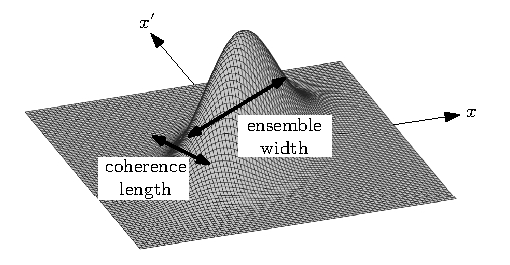
\includegraphics[width=.7\linewidth]{figures/ch03_fig04.pdf}
\caption{Gaussian密度行列(3.79)の記述に関係する、主な量のいくつかの図解。密度行列の非対角方向$x=-x'$における広がりは、系が空間的干渉効果を示しうる特徴的距離を測るコヒーレンス長$\ell(t)\equiv1/\sqrt{8A(t)}$で定量化される。アンサンブル幅$\Delta X(t)\equiv1/\sqrt{8C(t)}$は、異なる位置$x$についての確率分布$P(x,t)\equiv\rho_{\mathrm S}(x,x,t)$の大きさを表す。}\label{fig:3.4}
\end{figure}

% 原文 p.141
\hypertarget{srcpage:141}{}\label{srcpage:141}
他方、$\rho_{\mathrm S}(x,x',t)$の対角方向$x=x'$での幅は、確率分布$P(x,t)\equiv\rho_{\mathrm S}(x,x,t)$の大きさに対応する。この分布は、位置測定で系が$x$に見いだされる確率を記述する。この幅は$\sqrt{C(t)}$に反比例する［(3.79)参照］。したがって、位置空間アンサンブルの全体の大きさを定量化するアンサンブル幅$\Delta X(t)$を
\begin{equation}
\Delta X(t)=\frac{1}{\sqrt{8C(t)}}
\tag{3.81}
\end{equation}
と導入する。

係数$B(t)$は、$A(t)$および$C(t)$とともに、運動量分布の幅$\Delta P(t)$に関係し、これは
\begin{equation}
\Delta P(t)=\sqrt2\left[A(t)+\frac{B^2(t)}{4C(t)}\right]^{1/2}
\tag{3.82}
\end{equation}
で与えられる。(3.81)、(3.82)を用いると、対応する不確定性関係は
\begin{equation}
\Delta X(t)\Delta P(t)=\frac12\left[\frac{A(t)}{C(t)}+\frac{B^2(t)}{4C(t)}\right]^{1/2}
\tag{3.83}
\end{equation}
と書ける。最後に、項$D(t)$は、密度行列のトレースが常に保存されることを保証する。

Gaussian型の仮定(3.79)を運動方程式(3.78)に代入すると、係数$A(t)$、$B(t)$、$C(t)$、$D(t)$についての連立微分方程式が得られ、任意の初期条件に対して具体的に解ける（例えば文献\cite{ref017}の付録A2を参照）。ここでは、特定の初期状態、すなわち$x=0$を中心とする幅$b$の純粋状態のGaussian波束
\begin{equation}
\psi(x,0)=\left[\frac{1}{2\pi b^2}\right]^{1/4}\exp\left(\frac{-x^2}{4b^2}\right)
\tag{3.84}
\end{equation}
を選び、縮約密度行列のデコヒーレンスの動力学を示そう。これから初期密度行列
\begin{equation}
\rho_{\mathrm S}(x,x',0)=\left[\frac{1}{2\pi b^2}\right]^{1/2}\exp\left(-\frac{x^2+x'^2}{4b^2}\right)
\tag{3.85}
\end{equation}
を得る。これは(3.79)に現れる係数について、初期値$A(0)=C(0)=1/8b^2$、$B(0)=D(0)=0$に対応する。

密度行列(3.85)を図3.5に示す。Gaussianは$x$軸と$x'$軸に関して対称であり、すなわちコヒーレンス長とアンサンブル幅の大きさが等しい。この初期状態(3.85)に対して、係数$A(t)$、$B(t)$、$C(t)$、$D(t)$の時間依存性は容易に計算できる。$A(t)$、$C(t)$の表式を具体的に書けば（導出は文献\cite{ref007}、または文献\cite{ref017}の付録A2を参照）、
\begin{equation}
A(t)=\frac{\Lambda t^3+3m^2b^2/2+2\Lambda^2b^2t^4+12\Lambda m^2b^4t}{3t^2+8\Lambda b^2t^3+12m^2b^4}
\tag{3.86}
\end{equation}
および
\begin{equation}
C(t)=\frac12\left[\frac{t^2}{m^2b^2}+\frac83\frac{\Lambda t^3}{m^3}+4b^2\right]^{-1}
\tag{3.87}
\end{equation}
となる。
\begin{figure}[htbp]\centering
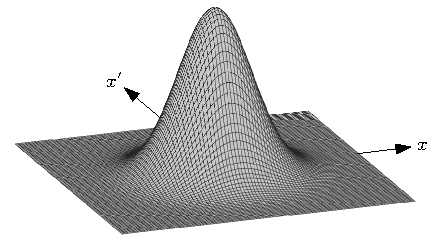
\includegraphics[width=.7\linewidth]{figures/ch03_fig05.pdf}
\caption{初期密度行列$\rho_{\mathrm S}(x,x',0)$［(3.85)参照］の図解。密度行列は$(x,x')$平面で対称なGaussianの形をもち、コヒーレンス長$\ell(0)$（「非対角」$x=-x'$に沿う広がり）が、アンサンブル幅$\Delta X(0)$（対角$x=x'$に沿う幅）に等しい。}\label{fig:3.5}
\end{figure}

% 原文 p.142
\hypertarget{srcpage:142}{}\label{srcpage:142}
コヒーレンス長、アンサンブル幅、縮約密度行列の純度などの主要な関連量の時間発展を調べる前に、環境散乱によるデコヒーレンスを考慮したとき、初期Gaussian(3.85)が時間とともにどのように発展すると予想されるかを、簡単に論じよう。環境との相互作用によって、与えられた距離$\Delta x=|x-x'|$にわたる空間的コヒーレンスの観測が、ますます難しくなると予想される。すなわち、コヒーレンス長$\ell(t)$［(3.80)参照］は時間とともに減少し、「古典的」対角線$x=x'$に垂直な方向にGaussian(3.85)を「絞る」と期待される。完全なデコヒーレンスの極限では、Gaussianは、対角線$x=x'$に沿う無限に細い稜線という、準古典的分布の形に近づくだろう。同時に、$x=-x'$方向の絞り込みに伴って、$x=x'$方向には広がると予想される。

係数$A(t)$、$C(t)$の具体的な表式(3.86)、(3.87)を用い、関連する量の時間発展を調べて、これらの直観を確認しよう。デコヒーレンスについて最も関心がある量は、おそらく(3.80)で定義したコヒーレンス長$\ell(t)$である。(3.86)を用いると、その時間依存性は
\begin{equation}
\ell(t)=\frac{1}{\sqrt{8A(t)}}=\frac12\left[\frac{3t^2+8\Lambda b^2t^3+12m^2b^4}{2\Lambda t^3+3m^2b^2+4\Lambda^2b^2t^4+24\Lambda m^2b^4t}\right]^{1/2}
\tag{3.88}
\end{equation}
で与えられる。

% 原文 p.143
\hypertarget{srcpage:143}{}\label{srcpage:143}
予想どおり、$t=0$でコヒーレンス長は波束の幅$b$に等しい。環境との相互作用がない場合（$\Lambda=0$）、$\ell(t)$は
\begin{equation}
\ell_{\mathrm{free}}(t)=\frac12\left[\frac{t^2}{m^2b^2}+4b^2\right]^{1/2}=\Delta X_{\mathrm{free}}(t)
\tag{3.89}
\end{equation}
となる。この表式は、本章の初めで論じた波束の自由なコヒーレント拡散を記述するにすぎない。これは、$\sigma\equiv\sqrt2b$と明らかに同定すれば、(3.3)に相当する（本節では$\hbar\equiv1$と置いたことも思い出そう）。

$\ell(t)$［(3.88)参照］の時間発展を詳しく調べよう。以下では、時間を$\tau_b\equiv1/\Lambda b^2$の単位で測る。これは、距離$\Delta x=b$（波束の初期幅）にわたる空間的コヒーレンスの特徴的な局在化時間尺度である。$\ell(t)$のグラフを図3.6に示す。

まず、局在化時間尺度$\tau_b$よりはるかに短い時刻$t$での$\ell(t)$の時間発展を調べよう。(3.88)を$\Lambda b^2t=0$のまわりで$\Lambda b^2t$の1次まで展開すると
\begin{equation}
\ell(t)\approx b(1-4\Lambda b^2t)
\tag{3.90}
\end{equation}
を得る。したがって、環境散乱の影響により、短時間ではコヒーレンス長は時間に対して線形に減少し、その減少率は散乱定数$\Lambda$に比例することがわかる。
\begin{figure}[htbp]\centering
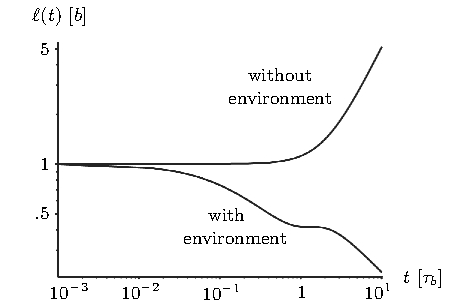
\includegraphics[width=.7\linewidth]{figures/ch03_fig06.pdf}
\caption{Joosら\cite{ref017}が調べたGaussian波束について、(3.88)で与えられるコヒーレンス長$\ell(t)$の時間依存性。時間$t$は特徴的な局在化時間尺度$\tau_b=1/\Lambda b^2$を単位として測り、$\ell(t)$は波束の初期幅$\ell(0)=b$を単位として表示した。上の曲線は環境との相互作用がない場合（$\Lambda=0$）の振る舞いを示す。下の曲線は環境散乱の効果を示し、系が空間的コヒーレンスを維持できる距離が時間とともに急速に減少することを示している。}\label{fig:3.6}
\end{figure}

% 原文 p.144
\hypertarget{srcpage:144}{}\label{srcpage:144}
一方、$t$が局在化時間尺度$\tau_b$よりはるかに長い極限も考えられる。巨視的物体の散乱率$\Lambda$が非常に大きな値を取りうること（表3.1参照）を考えれば、この極限が適用されるために$t$自体が大きい必要はない。例えば、大きさ$a=10^{-3}\,\mathrm{cm}$の塵粒子に対し、$\Lambda\approx10^{20}\,\mathrm{cm}^{-2}\,\mathrm s^{-1}$というかなり低い値を用い、初期のコヒーレントな広がりを大きさの10\%、すなわち$b=10^{-4}\,\mathrm{cm}$としても、$\tau_b\approx10^{-12}\,\mathrm s$を得る。したがって、巨視的物体では、通常、1秒に満たないごく短い時間で$t\gg\tau_b$の極限に達する。この極限では、(3.88)は漸近表式
\begin{equation}
\ell(t)\longrightarrow\frac{1}{\sqrt{2\Lambda t}}
\tag{3.91}
\end{equation}
に近づく。したがって、この場合のコヒーレンス長は$t^{-1/2}$に従い、初期状態(3.84)の幅$b$には依存しない。

次に、アンサンブル全体の大きさ$\Delta X(t)$の時間発展を考えよう。(3.81)、(3.87)から
\begin{equation}
\Delta X(t)=\frac{1}{\sqrt{8C(t)}}=\frac12\left[\frac{t^2}{m^2b^2}+\frac83\frac{\Lambda t^3}{m^3}+4b^2\right]^{1/2}
\tag{3.92}
\end{equation}
を得る。環境との相互作用がない場合（$\Lambda=0$）、すなわち初期波動関数(3.84)で記述される自由粒子の純粋にユニタリーな時間発展では、$\Delta X(t)$は$\Lambda=0$で評価したコヒーレンス長$\ell(t)$の表式［(3.89)参照］と一致し、
\begin{equation}
\Delta X_{\mathrm{free}}(t)=\frac12\left[\frac{t^2}{m^2b^2}+4b^2\right]^{1/2}
\tag{3.93}
\end{equation}
となる。したがって、環境がなければ、広がりは、位置のアンサンブルを記述する$x=x'$方向と、空間的コヒーレンスを表す$x=-x'$方向で、まったく同じ速さで進む。これは、もちろん自由粒子に予想される振る舞いである。環境が存在しなければ、一方の方向を他方に対して特別扱いする物理的機構は存在しない。しかし、環境を含めると非対称性が導入される。散乱事象は、系の位置を測る一種の測定装置として働くようになる。大まかにいえば、散乱粒子は、二つの位置の和$(x+x')$には鈍感なまま、二つの位置$x$、$x'$の差$|x-x'|$を識別しようとする。座標$(x+x')$と$(x-x')$に関する環境監視過程のこの非対称性は、$\rho_{\mathrm S}(x,x',t)$の運動方程式の形［(3.78)の右辺参照］にまとめられており、(3.92)と(3.88)の比較からわかるように、$\Delta X(t)$と$\ell(t)$の異なる時間発展をもたらす。

% 原文 p.145
\hypertarget{srcpage:145}{}\label{srcpage:145}
環境相互作用が存在すると、(3.92)の余分な項$\frac83\frac{\Lambda t^3}{m^3}$により、アンサンブルの幅は時間とともにいっそう速く増大する（図3.7参照）。\footnote{一見すると、驚くべき結果に思えるかもしれない。本章の導入では、デコヒーレンスは波束の拡散に対抗すると述べたのだから。しかし、ここには矛盾はない。肝心なのは、コヒーレントな拡散とアンサンブルの拡散の違いを念頭に置くことである。コヒーレントな拡散とは、例えば干渉実験を行うことによって、系が、ますます大きく離れた位置の重ね合わせにあるとわかることを意味する。これに対し、アンサンブルの拡散は、位置測定で系を見いだしうる位置の範囲が増大することに対応するだけである。}この模型で、環境の存在がこの「古典的」拡散を加速するのは、散乱事象によって系の平均エネルギーが増加するためである。このエネルギー増加は、散乱事象によって系に反跳が生じないという仮定の帰結である（121ページ参照）。

こうして、密度行列の時間発展は、図3.8に示すように、二つの逆向きの影響の競合として視覚化できる。一方では、自由粒子のユニタリーな発展と、散乱事象による平均エネルギーの増加の両方によって、位置空間アンサンブル全体の空間的広がり$\Delta X(t)$が、時間とともにますます広がる。他方、同じ散乱事象は系の位置の連続的監視としても働き、コヒーレンス長$\ell(t)$を減少させ、したがって次第に短い距離にわたる空間的コヒーレンスまで抑制する。
\begin{figure}[htbp]\centering
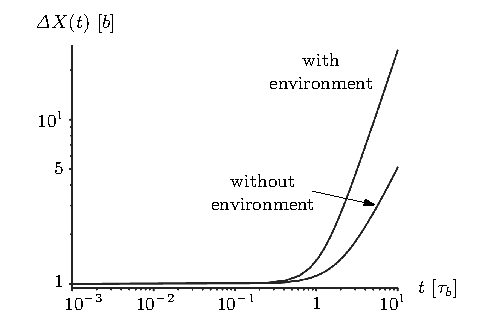
\includegraphics[width=.7\linewidth]{figures/ch03_fig07.pdf}
\caption{Joosら\cite{ref017}が調べたGaussian波束について、(3.92)で与えられるアンサンブル幅$\Delta X(t)$の時間発展。時間$t$は特徴的な局在化時間尺度$\tau_b=1/\Lambda b^2$を単位として測り、$\Delta X(t)$は波束の初期幅$\Delta X(0)=b$を単位として示した。}\label{fig:3.7}
\end{figure}
% 原文 p.146
\hypertarget{srcpage:146}{}\label{srcpage:146}
\begin{figure}[htbp]\centering
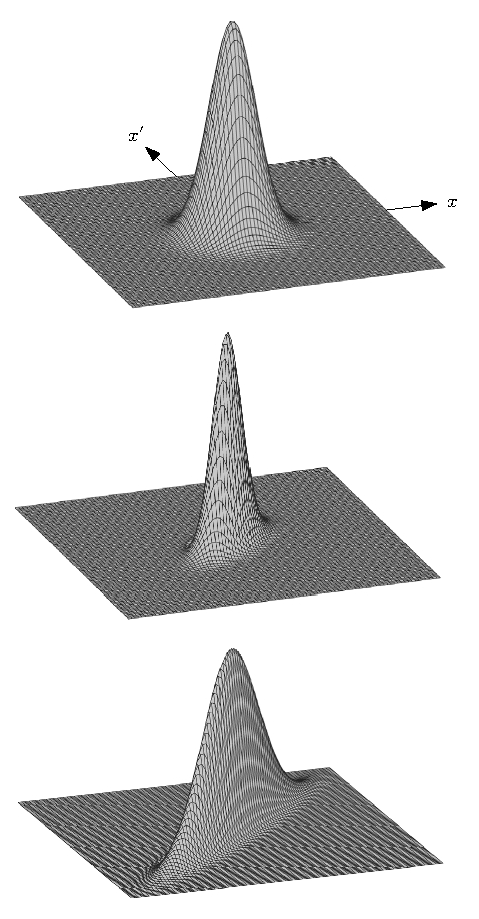
\includegraphics[width=.63\linewidth]{figures/ch03_fig08.pdf}
\caption{散乱環境の影響下における、(3.85)の初期状態をもつGaussian波束(3.79)の時間発展。(3.79)の係数$A(t)$、$C(t)$は、それぞれ(3.86)、(3.87)によって定まる。空間的コヒーレンスを表す非対角方向$x=-x'$におけるGaussianの幅は次第に縮まり、密度行列は対角線$x=x'$に集中した準古典的な位置の確率分布に近づく。}\label{fig:3.8}
\end{figure}

% 原文 p.147
\hypertarget{srcpage:147}{}\label{srcpage:147}
コヒーレンス長$\ell(t)$の減少と、アンサンブルの大きさ$\Delta X(t)$の増大の相互作用を定量化するため、両者を組み合わせた無次元量として、しばしば比
\begin{equation}
\delta(t)\equiv\frac{\ell(t)}{\Delta X(t)}=\sqrt{\frac{C(t)}{A(t)}}
\tag{3.94}
\end{equation}
を考える（例えば文献\cite{ref017,ref173}）。$\delta(t)$のグラフを図3.9に示す。環境がなければ$\delta(t)$は一定である。すなわち、コヒーレントな拡散は$x=x'$方向と$x=-x'$方向で同じ速さで進む［(3.89)とそれに続く議論を参照］。環境を含めると、コヒーレンス長$\ell(t)$は減少する一方、全体の幅$\Delta X(t)$は増大する。しかし、$\Delta X(t)$の増大率は$\ell(t)$の減少率より遅く、結果として$\delta(t)$は減少する。

量$\delta(t)$を導入したもう一つの理由は、別のデコヒーレンスの尺度、すなわち2.4.3節で導入した密度行列$\hat\rho$の純度$\varsigma=\operatorname{Tr}(\hat\rho^2)$［(2.30)参照］と、容易に直接結びつけられることである。この模型の縮約密度行列$\rho_{\mathrm S}(t)$の純度は
\begin{equation}
\varsigma(t)=\sqrt{\frac{C(t)}{A(t)}}
\tag{3.95}
\end{equation}
となる。しかし、これは明らかに$\delta(t)$の表式(3.94)と一致する。すなわち、量$\delta(t)$は、散乱模型の縮約密度行列の純度も記述する。図3.9から、予想どおり環境散乱は縮約密度行列の純度を減少させ、デコヒーレンスの漸進的な作用を反映することがわかる。
\begin{figure}[htbp]\centering
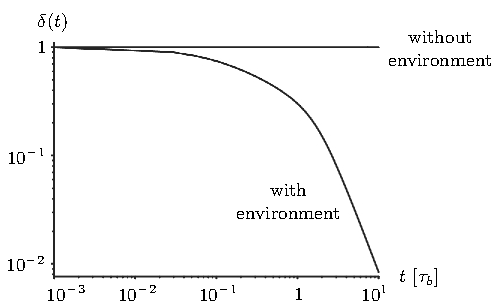
\includegraphics[width=.7\linewidth]{figures/ch03_fig09.pdf}
\caption{環境散乱がある場合とない場合の比$\delta(t)\equiv\ell(t)/\Delta X(t)$［(3.94)参照］の時間依存性。量$\delta(t)$は、この模型の局所密度行列の純度の時間発展も記述する。ここでも時間$t$は、特徴的な局在化時間尺度$\tau_b=1/\Lambda b^2$を単位として測る。}\label{fig:3.9}
\end{figure}

% 原文 p.148
\hypertarget{srcpage:148}{}\label{srcpage:148}
最後に、それぞれ$x=\pm x_0$を中心とする、(3.84)の形の二つのGaussian波束の、等しい重みをもつ重ね合わせ
\begin{equation}
\begin{aligned}
\Psi(x,0)&=\psi_{x_0}(x,0)+\psi_{-x_0}(x,0)\\
&=\left[\frac{1}{2\pi b^2}\right]^{1/4}\left\{\exp\left(\frac{-(x-x_0)^2}{4b^2}\right)+\exp\left(\frac{-(x+x_0)^2}{4b^2}\right)\right\}
\end{aligned}\tag{3.96}
\end{equation}
の時間発展を示そう。この波動関数を図3.10に示す。

$x_0\gg b$であれば、このような量子状態は、距離$2x_0$離れた明確で区別可能な二つの位置の重ね合わせによって粒子が記述される、非古典的な状況に対応する。対応する密度行列は
\begin{equation}
\begin{aligned}
\rho_{\mathrm S}(x,x',0)&=\Psi^*(x',0)\Psi(x,0)\\
&=\psi_{x_0}^*(x',0)\psi_{x_0}(x,0)+\psi_{-x_0}^*(x',0)\psi_{-x_0}(x,0)\\
&\quad+\psi_{x_0}^*(x',0)\psi_{-x_0}(x,0)+\psi_{-x_0}^*(x',0)\psi_{x_0}(x,0)
\end{aligned}\tag{3.97}
\end{equation}
である。この密度行列を、図3.11の最上段に示す。非対角線$x=-x'$に沿う二つのピークは、(3.96)で導入した二つの波束$\psi_{x_0}(x,0)$、$\psi_{-x_0}(x,0)$の間の空間的干渉項$\psi_{x_0}^*(x',0)\psi_{-x_0}(x,0)$、$\psi_{-x_0}^*(x',0)\psi_{x_0}(x,0)$に対応する。

運動方程式(3.78)で決まる、密度行列(3.97)のその後の時間発展を、図3.11に示す。予想どおり、$x=\pm x_0$のまわりの二つの領域の間の空間的コヒーレンスに対応する干渉項は、環境の存在によって次第に抑制される。完全なデコヒーレンスの極限では、それぞれ$+x_0$、$-x_0$のまわりへの系の局在化を記述する、二つの状態の（ただし非真正な！）アンサンブルを得る。すなわち、系だけに関係する測定では、このアンサンブルを、対応する局在した位置の古典的な（真正な）アンサンブルと区別できない。
\begin{figure}[htbp]\centering
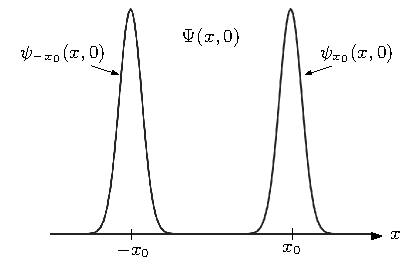
\includegraphics[width=.65\linewidth]{figures/ch03_fig10.pdf}
\caption{それぞれ$+x_0$、$-x_0$を中心とする、二つのGaussian波束の重ね合わせ(3.96)の図解。}\label{fig:3.10}
\end{figure}
% 原文 p.149
\hypertarget{srcpage:149}{}\label{srcpage:149}
\begin{figure}[htbp]\centering
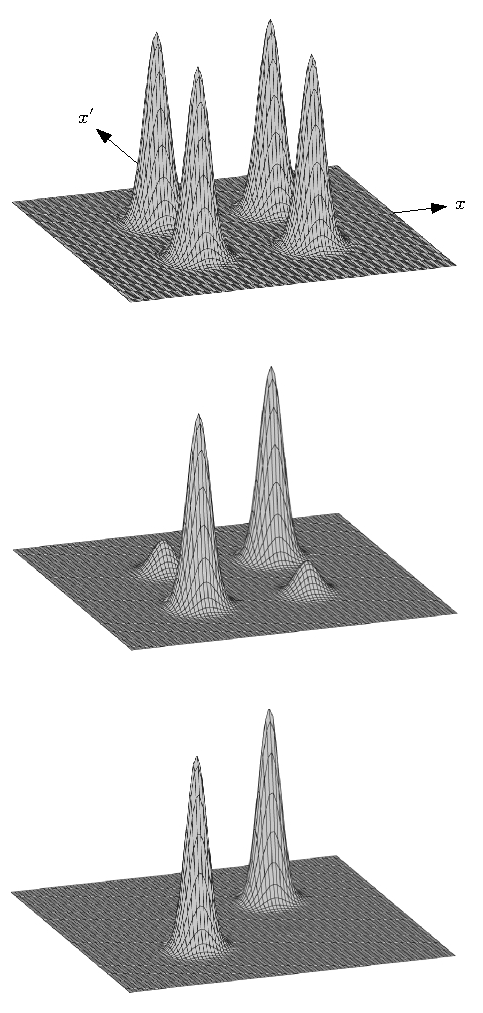
\includegraphics[width=.63\linewidth]{figures/ch03_fig11.pdf}
\caption{二つのGaussian波束の重ね合わせ(3.96)についての、密度行列$\rho_{\mathrm S}(x,x',t)$の時間発展。非対角線$x=-x'$に沿う干渉項が、環境粒子の散乱によって次第に減衰する。}\label{fig:3.11}
\end{figure}

% 原文 p.150
\hypertarget{srcpage:150}{}\label{srcpage:150}
\subsectionlink{まとめ}
環境粒子の散乱は、巨視的領域における主要なデコヒーレンス源の一つであり、したがって、身の回りの日常世界に古典性が出現するうえで、きわめて重要な役割を果たす。散乱によるデコヒーレンスは、例えば、環境が系の位置の連続的監視装置として働くことの帰結としてデコヒーレンスを理解するという、基本的な概念面を説明するのにも、まさに適している。

一回の散乱事象が不完全な経路情報しか環境に符号化しない場合（「長波長極限」）、空間的干渉項は［(3.57)参照］
\begin{equation}
\rho_{\mathrm S}(\bm x,\bm x',t)=\rho_{\mathrm S}(\bm x,\bm x',0)e^{-\Lambda(\bm x-\bm x')^2t}
\tag{3.98}
\end{equation}
に従って指数関数的に減衰することがわかった。散乱定数$\Lambda$は、散乱過程の具体的な物理的性質を担っている。したがって、距離$\Delta x=|\bm x-\bm x'|$にわたる空間的干渉のデコヒーレンスの特徴的時間尺度$\tau_{\Delta x}$は［(3.58)参照］
\begin{equation}
\tau_{\Delta x}=\frac{1}{\Lambda(\Delta x)^2}
\tag{3.99}
\end{equation}
である。$\tau_{\Delta x}$は、コヒーレントな隔たり$\Delta x$に対して二次的に減少する。この隔たりが環境粒子の典型的な波長より大きくなると、一回の散乱事象で完全に識別されるようになる。それに伴って、デコヒーレンス率は飽和し、全散乱率だけで与えられる［(3.48)参照］。

また、典型的なデコヒーレンス時間尺度の具体的な数値もいくつか見積もり、散乱によるデコヒーレンスの有効性と遍在性を印象的に示した。一見すると、系を環境から適切に遮蔽すれば、デコヒーレンスを完全に避けられると思ったかもしれない。しかし、見てきたように、実際には、そのような完全な遮蔽を達成することは不可能である。利用できる最良の実験室真空でさえ、空気分子の密度は、巨視的な空間的干渉を強く、事実上瞬時に減衰させるほど大きい。仮に周囲の気体分子が系と相互作用することを完全に防げたとしても、熱光子が急速なデコヒーレンスを引き続き生じさせるだろう。さらにその効果を小さくできても、逃れられない太陽ニュートリノとマイクロ波背景放射の環境によるデコヒーレンスは、なお生じる。これらの議論は、巨視的尺度において位置が遍在的な優先基底となる理由（また、2.8.4節で述べたキラル分子など、しばしば微視的尺度でもそうなる理由）も示している。

% 原文 p.151
\hypertarget{srcpage:151}{}\label{srcpage:151}
量子系を散乱環境の影響から遮蔽することは実際には不可能であり、こうした散乱過程が系の運動と観測可能な量子特性に決定的な影響を与えるという認識は、波束を、身の回りにある空間的に広がった物体と直接同一視する真の「波動力学」を目指したSchrödingerの試みに、欠けていた重要な要素を与えた。散乱環境に接している物体を記述する縮約密度行列を用いれば、次第に減少するコヒーレンス長によって幅が与えられる波束の、非真正なアンサンブルを定義できる。そのような個々の波束を、少なくとも局所測定という操作的な意味では、よく局在した粒子の現れと同一視できる。

6.2節で詳しく論じるように、大きな分子を用いた最近の二重スリット型実験によって、散乱によるデコヒーレンス模型の定性的・定量的な予測を、直接確認できるようになった。この種の実験が、いっそう大きな物体に干渉縞を生成し、デコヒーレンスの漸進的な影響を観測する方向へ進むにつれて、実験室で、ますます巨視的な尺度において、これらの模型を直接検証できるようになるだろう。
